\documentclass[10pt,twoside]{book}
\usepackage[utf8]{inputenc}
\usepackage[latin,spanish]{babel}
\usepackage[T1]{fontenc}
\usepackage{fontspec}
\usepackage{blindtext}
\usepackage{hyperref}
\hypersetup{
    hidelinks,
    pdftitle={Santo Rosario y \'Angelus},
    pdfauthor={Sergio},
    pdfkeywords={Cat\'olico, Santa Mar\'ia, Santo Rosario},
    pdfcreator={VS Code + LuaTeX}
}
\usepackage[spanish]{cleveref}
\usepackage{setspace}
\usepackage{multicol}
\usepackage{biblatex}
\addbibresource{biblio.bib}
\usepackage{geometry}
\geometry{
    a4paper,
    inner=20mm,
    outer=10mm,
    top=15mm,
    bottom=15mm
}
\usepackage{paracol}
\usepackage{lettrine}
\usepackage{xcolor}
\usepackage{gregoriotex}
\usepackage{graphicx}
\graphicspath{ {images/} }
\usepackage{fancyhdr}
\pagestyle{fancy}
\fancyhf{}
\fancyfoot[LE,RO]{\thepage}
\renewcommand{\headrulewidth}{0pt}
\renewcommand{\footrulewidth}{0pt}

\setlength{\columnseprule}{0.4pt}
\colseprulecolor{red}
\setlength{\columnseprule}{0.4pt}
\def\columnseprulecolor{\color{red}}

\usepackage{datetime}
\newdateformat{monthyeardate}{%
  \monthname[\THEMONTH] \THEYEAR
}
\newcommand{\primeraletragranderoja}[2]{
    \lettrine[lines=2]{\textcolor{red}{#1}}{#2}
}

\newcommand{\primeraletragranderojasola}[1]{
    \lettrine[lines=2]{\textcolor{red}{#1}}{}
}

\newcommand{\primeraletragrande}[2]{
    \lettrine[lines=2]{#1}#2
}

\newcommand{\letraroja}[2]{
    \textcolor{red}{#1}#2
}

\newcommand{\versiculo}[1]{
    \textcolor{red}{\Vbar.} #1.
}

\newcommand{\respuesta}[1]{
    \textcolor{red}{\Rbar.} #1.
}

\newcommand{\textopequenorojo}[1]{
    {\textcolor{red}{\small{#1}}}
}

\newcommand{\versiculorespuesta}[2]{
    \versiculo{#1}\\
    \respuesta{#2}
}

\newcommand{\versiculorespuestaseguido}[2]{
    \versiculo{#1}\respuesta{#2}
}

\newcommand{\redcross}{
    \textcolor{red}{\grecross}
}

\newcommand{\lineahorizontal}[2]{
    \begin{center}
        {\rule{#1cm}{#2pt}}
    \end{center}
}

\newcommand{\lineahorizontalroja}[2]{
    \begin{center}
        \textcolor{red}{\rule{#1cm}{#2pt}}
    \end{center}
}

\newcommand{\latinderecha}[1]{
    \begin{otherlanguage}{latin}
        \begin{rightcolumn}
            \input{#1}    
        \end{rightcolumn}
    \end{otherlanguage}
}

\newcommand{\castellanoizquierda}[1]{
    \begin{leftcolumn}
        \input{#1}
    \end{leftcolumn}
}

\newcommand{\castellanoizquierdasincro}[1]{
    \begin{leftcolumn*}
        \input{#1}
    \end{leftcolumn*}
}

\newcommand{\castellanoizquierdasincronota}[2]{
    \begin{leftcolumn*}[#1]
        \input{#2}
    \end{leftcolumn*}
}

\newcommand{\filacastellanolatin}[2]{
    {    
        \begin{leftcolumn}
            \input{#1}
        \end{leftcolumn}
        \begin{otherlanguage}{latin}
            \begin{rightcolumn}
                \input{#2}    
            \end{rightcolumn}
        \end{otherlanguage}
    }
}

\newcommand{\filacastellanolatinsincro}[2]{
    {    
        \begin{leftcolumn*}
            \input{#1}
        \end{leftcolumn*}
        \begin{otherlanguage}{latin}
            \begin{rightcolumn}
                \input{#2}    
            \end{rightcolumn}
        \end{otherlanguage}
    }
}

\newcommand{\filacastellanolatinsincronota}[3]{
    \castellanoizquierdasincronota{#1}{#2}
    \latinderecha{#3}
}

\newcommand{\titulomisterios}[2]{
    {    
        \begin{minipage}[t]{0.595\textwidth}
            \subsection*{#1}
        \end{minipage}\begin{minipage}[t]{0.395\textwidth}
            \begin{flushright}
                \textcolor{red}{#2}
            \end{flushright}
        \end{minipage}
    }
}

\newcommand{\titulomisterio}[2]{
    {
        \begin{minipage}[t]{0.595\textwidth}
            \section*{#1}
        \end{minipage}\begin{minipage}[t]{0.395\textwidth}
            \begin{flushright}
                \textcolor{red}{#2}
            \end{flushright}
        \end{minipage}
    }
}

\newcommand{\iralfinal}{
    \begin{center}
        \textcolor{red}{Una vez terminamos nos vamos a la \cpageref{final-prayer} para las oraciones finales.}
    \end{center}
}





\begin{document}

\begin{titlepage}
      \begin{center}

            \vspace*{10em}

            {\Huge \uppercase{Santo Rosario, Semana Santificada y Ángelus}}

            \vspace{1.5em}

            {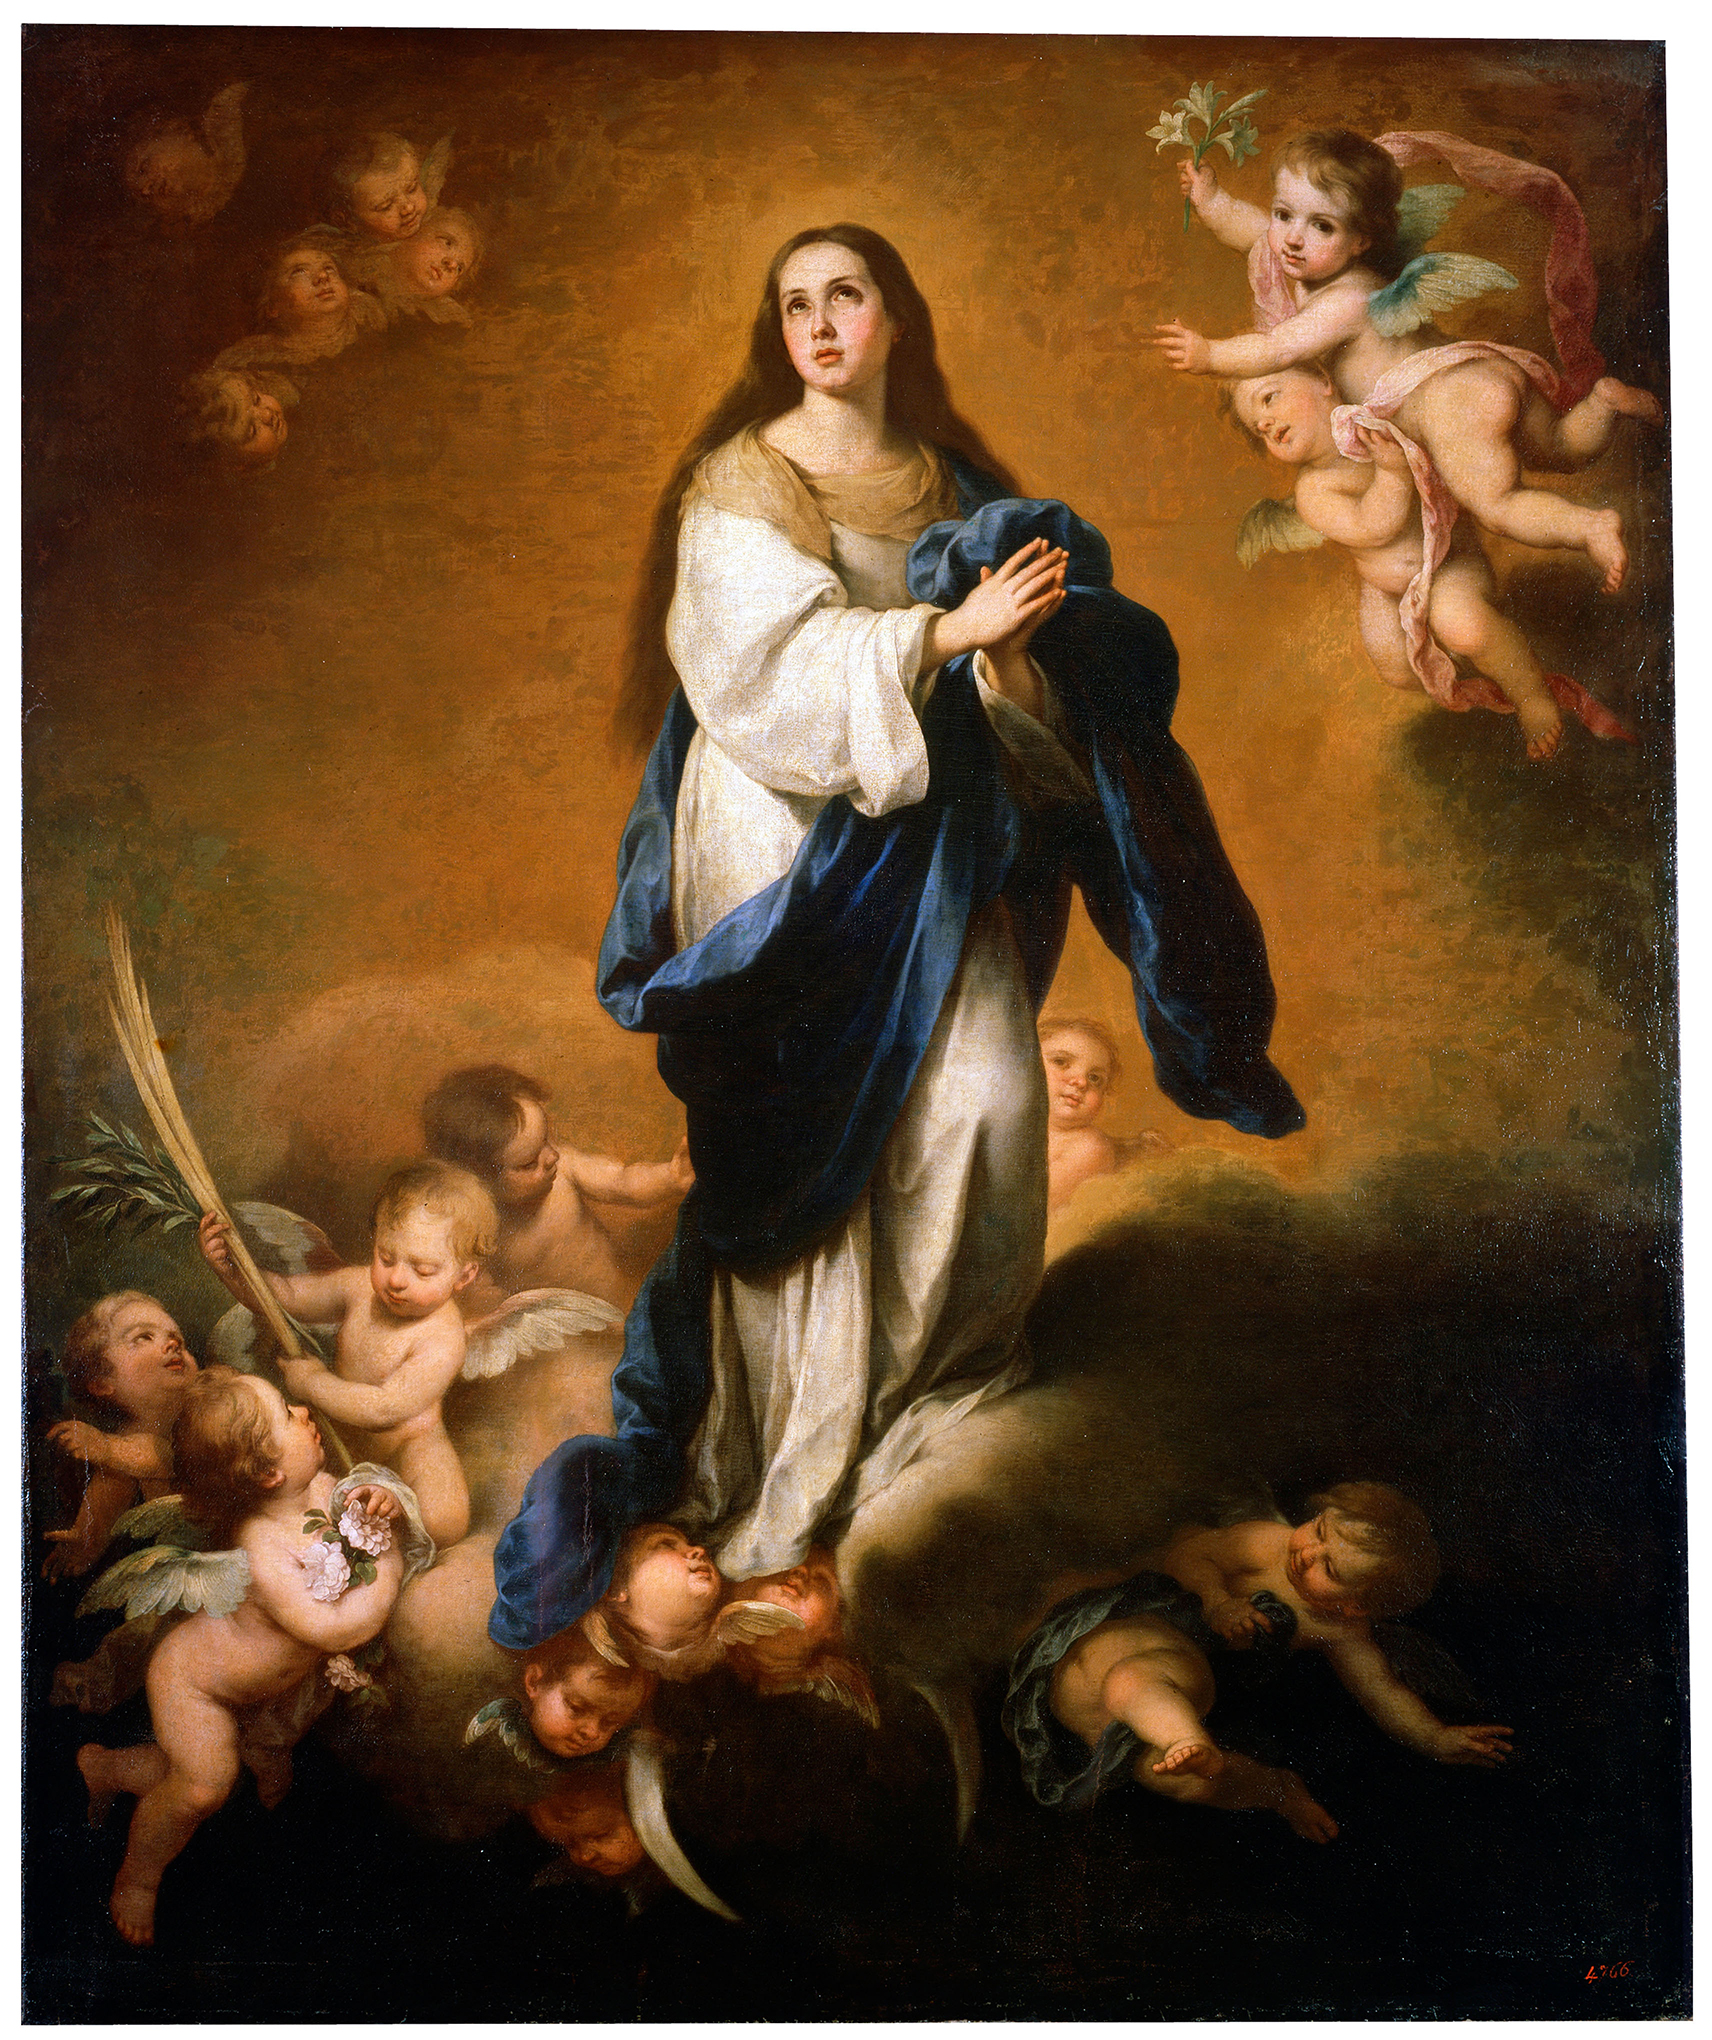
\includegraphics[scale=0.95]{foto-04.jpg}}

            \vspace{0.5em}

            Sergio

            Valladolid (España), \monthyeardate\today
      \end{center}
\end{titlepage}
\twosided{c}
\footnotelayout{m}

\chapter*{\centering\textcolor{red}{S}anto \textcolor{red}{R}osario \textcolor{red}{M}editado \\ y \\ \textcolor{red}{S}emana \textcolor{red}{S}antificada\footnote{Todos los pasajes
bíblicos han sido sacados de \cite{bover-cantera}}}

\begin{paracol}{2}

      \ensurevspace{20mm}

      \begin{leftcolumn}
            En el Nombre del Padre, y del{\redcross}Hijo, y del Espíritu Santo. Amén.
      \end{leftcolumn}
      \begin{otherlanguage}{latin}
            \begin{rightcolumn}
                  In Nómine Pátris, et{\redcross}Filii, et Spíritus Sancti. Amen    
            \end{rightcolumn}
      \end{otherlanguage}

      \begin{leftcolumn*}[\centering\textcolor{red}{Acto de contrición\footnote{En vez del \textit{Señor mio, Jesucristo} o del \textit{Confíteor}, podemos rezar\cite{compendio}: \textcolor{red}{D}ios mío, me arrepiento de todo corazón de todos mis pecados y los aborrezco, porque al pecar, no sólo merezco las penas establecidas 
por ti justamente, sino principalmente porque te ofendí, a ti sumo Bien y digno de amor por encima de todas las cosas. Por eso propongo firmemente, 
con ayuda de tu gracia, no pecar más en adelante y huir de toda ocasión de pecado. Amén.|| Latín: \textcolor{red}{D}eus meus, ex toto corde p{\ae}nitet me ómnium meórum peccatórum, éaque detéstor, quia peccándo, non solum pœnas a te iuste statútas 
proméritus sum, sed pr{\ae}sértim quia offéndi te, summum bonum, ac dignum qui super ómnia diligáris. Ídeo fírmiter propóno, adiuvánte grátia tua, 
de cétero me non peccatúrum peccandíque occasiónes próximas fugitúrum. Amen.}}\vspace{0.5em}]
            \primeraletragranderoja{S}{eñor}mío Jesucristo, Dios y Hombre verdadero, Creador y Redentor mío: por ser vos quién sois, y porque os amo sobre todas las cosas,
me pesa de todo corazón de haberos ofendido, propongo firmemente nunca más pecar, y apartarme de todas las ocasiones de ofenderos,
confesarme, y cumplir la penitencia que me fuere impuesta; ofrézcoos mi vida, obras y trabajos en satisfacción de todos mis pecados;
y confío en vuestra bondad y misericordia infinita me los perdonaréis por los merecimientos de vuestra preciosísima sangre, pasión y muerte,
y me daréis gracia para enmendarme y para perseverar en vuestro santo servicio hasta el fin de mi vida. Amén.\cite{reyero}
      \end{leftcolumn*}
      \begin{otherlanguage}{latin}
            \begin{rightcolumn}
                \primeraletragranderoja{C}{onfíteor}Deo omnipoténti, beát{\ae} Marí{\ae} semper Virigini, beáto Michaéli Archángelo, beáto Joánni Baptíst{\ae}, sanctis 
Apóstolis Petro et Paulo, ómníbus Sanctis, quia peccávi nimis, cogitatióne, verbo et ópere, mea culpa, mea culpa, mea máxima culpa. Ideo precor beátam
Maríam semper Virgínem, beátum Michaélem Archángelum, beátum Joánnem Baptístam, sanctis Apóstolos Petrum et Paulum, omnes Sanctos,
oráre pro me ad Dóminum Deum nostrum.\\
Misereátur nostri omnipotens Deus, et, dimíssis peccátis nostris, perdúcat nos ad vitam {\ae}térnam. Amen.\\
Indulgéntiam, absolutionem, et remissiónem peccatórum nostrórum tríbuat nobis omnípotens et miséricors Dóminus. Amen.\cite{breviarium}
            \end{rightcolumn}
      \end{otherlanguage}

      \definecolumnpreamble{0}{\vspace{0.5em}}
      \definecolumnpreamble{1}{\vspace{0.5em}}

      \begin{leftcolumn*}
            \versiculorespuestaseguido{Abre, Señor, mis labios}{Y mi boca cantará tus alabanzas}
      \end{leftcolumn*}
      \begin{otherlanguage}{latin}
            \begin{rightcolumn}
                \versiculorespuestaseguido{Dómine, lábia mea apéries}{Et os meum annuntiábit laudem tuam}
            \end{rightcolumn}
      \end{otherlanguage}

      \begin{leftcolumn*}
            \versiculorespuestaseguido{Apresútare, Señor, a socorrerme}{Ven, oh Dios, en mi ayuda}
      \end{leftcolumn*}
      \begin{otherlanguage}{latin}
            \begin{rightcolumn}
                \versiculorespuestaseguido{Deum, in adjutórium meum inténde}{Dómine, ad adjuvándum me festina}
            \end{rightcolumn}
      \end{otherlanguage}

      \begin{leftcolumn*}
            \versiculorespuestaseguido{Gloria al Padre, al Hijo, y al Espíritu Santo}{Como era en el principio, ahora, y siempre, y por los siglos de los siglos. Amén}
      \end{leftcolumn*}
      \begin{otherlanguage}{latin}
            \begin{rightcolumn}
                \versiculorespuestaseguido{Glória Patri, et Filio, et Spirítui Sancto}{Sicut erat in princípio et nunc, et semper et in s{\ae}cula s{\ae}culórum. Amen}
            \end{rightcolumn}
      \end{otherlanguage}

      \begin{leftcolumn*}
            \versiculorespuestaseguido{María, Madre de gracia, Madre de Misericordia}{Defendednos del enemigo y amparadnos ahora y en la hora de nuestra muerte. Amén}
      \end{leftcolumn*}
      \begin{otherlanguage}{latin}
            \begin{rightcolumn}
                \versiculorespuesta{María Mater grati{\ae}, Mater Misericordi{\ae}}{Tu nos ab hoste protege et mortis hora súspice. Amen}
            \end{rightcolumn}
      \end{otherlanguage}
      \definecolumnpreamble{0}{\vspace{0em}}
      \definecolumnpreamble{1}{\vspace{0em}}
\end{paracol}

\vspace{0.5em}

\begin{center}
      \textcolor{red}{Decimos aquí las intenciones de este Rosario}
\end{center}

\vspace{-1em}

\begin{center}
      \section*{Dominica (Domingo)}

      \textbf{\textsl{\large Misterios Gloriosos}}
\end{center}

\vspace{0.5em}

\noindent\textbf{\textsc{I La Resurrección del Señor}}\hfill\textcolor{red}{Mt 28, 1-3.5-7}

\vspace{0.25em}

\lettrine[lines=2]{\textcolor{red}{P}}asado el sábado, ya para amanecer el día primero de la semana, vino María Magdalena con la otra María al sepulcro. Y sobrevino un gran terremoto,
pues un ángel del Señor bajó del cielo y acercándose removió la piedra del sepulcro y se sentó sobre ella. Era su aspecto como el relámpago, y su vestidura blanca como la nueve.
El ángel, dirigiéndose a las mujeres, dijo: No temáis vosotras, pues sé que buscáis a Jesús el crucificado. No está aquí; ha resucitado, según lo había dicho.
Venid y ved el sitio donde fue puesto. Id luego y decid a sus discípulos que ha resucitado de entre los muertos y que os precede a Galilea; allí le veréis.
Es lo que tenía que deciros.

\vspace{0.5em}

\begin{paracol}{2}
    \filacastellanolatin{oraciones/padrenuestro/castellano_sencillo.tex}{oraciones/padrenuestro/latin_sencillo.tex}
    \vspace{2mm}
    \filacastellanolatinsincronota{\textcolor{red}{El avemaría se repite 10 veces}}{oraciones/avemaria/castellano_sencillo.tex}{oraciones/avemaria/latin_sencillo.tex}
    \vspace{6mm}
    \filacastellanolatinsincro{oraciones/gloria/castellano_separado.tex}{oraciones/gloria/latin_separado.tex}
    \vspace{2mm}
    \filacastellanolatinsincro{oraciones/versiculos/maria_madre/castellano.tex}{oraciones/versiculos/maria_madre/latin.tex}
\end{paracol}

\vspace{0.75em}

\noindent\textbf{\textsc{II Las Ascensión Jesucristo a los cielos}}\hfill\textcolor{red}{Mc 16, 15-16.19-20}

\vspace{0.25em}

\lettrine[lines=2]{\textcolor{red}{Y}} les dijo: Id al mundo entero y predicad el Evangelio a toda la creación.
El que creyere y fuere bautizado, se salvará, mas el que no creyere, será condenado. Con esto el Señor Jesús, después de hablarles, fue elevado al cielo y se sentó a la diestra de Dios.
Y ellos, partiéndose de allí, predicaron por todas partes, cooperando el Señor y confirmando la palabra con las señales que la acompañaban.

\begin{center}
    Paternóster, diez Avemarías, Gloria

\end{center}

\begin{paracol}{2}
    \filacastellanolatin{oraciones/maria_madre/castellano_seguido.tex}{oraciones/maria_madre/latin_seguido.tex}
\end{paracol}

\vspace{0.75em}

\noindent\textbf{\textsc{III La Venida del Espíritu Santo sobre los Apóstoles}}\hfill\textcolor{red}{Act 2, 1-5}

\vspace{0.25em}

\lettrine[lines=2]{\textcolor{red}{M}}as el Paráclito, el Espíritu Santo, que enviará el Padre en mi nombre, Él os enseñará todas las cosas y os recordará todas las cosas que os dije yo.
Y al cumplirse el día de Pentecostés, estaban todos juntos en el mismo lugar. Y se produjo de súbito desde el cielo un estruendo como de viento que soplaba vehementemente,
y llenó toda la casa donde se hallaban sentados. Y vieron aparecer lenguas como de fuego, que, repartiéndose, se posaban sobre cada uno de ellos. Y se llenaron todos del Espíritu Santo,
y comenzaron a hablar en lenguas diferentes, según que el Espíritu Santo les movía a expresarse.

\begin{center}
    Paternóster, diez Avemarías, Gloria

\end{center}

\begin{paracol}{2}
    \filacastellanolatin{oraciones/maria_madre/castellano_seguido.tex}{oraciones/maria_madre/latin_seguido.tex}
\end{paracol}

\vspace{0.75em}

\noindent\textbf{\textsc{IV La Asunción de María Santísima a los cielos}}\hfill\textcolor{red}{Lc 1, 46-49; Apoc 11, 19}

\vspace{0.25em}

\lettrine[lines=2]{\textcolor{red}{M}}i alma magnifica al Señor y exulta de júbilo mi espíritu al Señor, mi Salvador, porque ha mirado la humildad de su sierva;
por eso todas las generaciones me llamarán bienaventurada, porque ha hecho en mi maravillas el Poderoso, cuyo nombre es santo. Y se abrió el templo de Dios, que está en el cielo,
y fué vista el arca de la alianza en el templo, y se produjeron relámpagos, y voces, y truenos, y temblor de tierra, y fuerte granizada.

\begin{center}
    Paternóster, diez Avemarías, Gloria

\end{center}

\begin{paracol}{2}
    \filacastellanolatin{oraciones/maria_madre/castellano_seguido.tex}{oraciones/maria_madre/latin_seguido.tex}
\end{paracol}

\vspace{0.75em}

% Cant 6,10; Apoc 12, 1; 18, 16; Ps 44, 10
\noindent\textbf{\textsc{V La Coronación de la Santísima Virgen María}}\hfill\textcolor{red}{Cant 6,10; Apoc 12, 1; 18, 16; Ps 44, 10}

\vspace{0.25em}

\lettrine[lines=2, ante={?`}]{\textcolor{red}{Q}}uién es esa que aparece resplandeciente como la aurora, hermosa cual luna, deslumbradora como el sol, imponente como batallones?.
Y una gran señal fué vista en el cielo: una Mujer vestida del sol, y la luna debajo de sus  pies, y sobre su cabeza una corona de doce estrellas.
Tiene Él escrito en su vestido y en su manto Rey de reyes y Señor de los que dominan. Está la Reina a su derecha, adornada con oro finísimo.

\begin{center}
    Paternóster, diez Avemarías, Gloria

\end{center}

\begin{paracol}{2}
    \filacastellanolatin{oraciones/maria_madre/castellano_seguido.tex}{oraciones/maria_madre/latin_seguido.tex}
\end{paracol}

\iralfinal

\begin{center}
      {\rule{10em}{0.4pt}}

      \vspace{0.75em}

      \textcolor{red}{Los domingos están dedicados a la Santísima Trinidad, para honrarla podemos rezar:}
\end{center}

\begin{multicols}{2}

      Santo, Santo, Santo, Señor Dios de los ejércitos. Llenos están los cielos y la tierra de vuestra gloria. Gloria al Padre, gloria al Hijo, gloria al Espíritu Santo. Amén.

\vspace{0.5em}

\noindent\textcolor{red}{Lectio i \hfill 2 Cor 13, 11.13}

\primeraletragranderoja{H}{ermanos:}Alegraos, sed perfectos, exhortaos, tened un mismo sentir, vivid en paz; y el Dios de la paz y de la caridad será con vosotros. La gracia de nuestro Señor Jesucristo,
y la caridad de Dios Padre, y la participación del Espíritu Santo sea con todos vosotros. Amén.

\vspace{0.5em}

\noindent\textcolor{red}{Lectio ii \hfill Rom 11, 33-36}

\primeraletragranderoja{O}{h}profundidad de las riquezas de la sabiduría y ciencia de Dios! {!`}Cuán inescrutables son sus juicios e incomprensibles sus caminos! Porque {?`}quién conoció los designios del Señor?,
o {?`}quién primero fué su consejero?, o {?`}quién primero le dió a Él, para que le sea recompensado? Porque de Él y por Él y en Él son todas las cosas; a Él sea gloria por todos los siglos.
Amén.

\vspace{0.5em}

\noindent\textcolor{red}{Lectio iii \hfill Dan 3, 55-56.52}

\primeraletragranderoja{B}{endito}eres, Señor, que penetras los abismos y estás sentado sobre Querubines. Bendito eres, Señor, en el firmamento del cielo, y digno de alabanza por todos los siglos
Aleluya, Aleluya. Bendito eres, Señor Dios de nuestros padres, y digno de alabanza por todos los siglos. Aleluia.

\vspace{0.5em}

\noindent\textcolor{red}{Lectio iv \hfill Mt 28, 18-20}

\primeraletragranderoja{D}{ijo}Jesús a sus discípulos: Se me ha dado poder en el cielo y en la tierra. Id, pues, y enseñad a todas las gentes, bautizándolas en el nombre del Padre y del Hijo y del Espíritu
Santo; enseñándoles a observar todo cuanto os he mandado. Y mirad que Yo estoy con vosotros todos los días hasta el fin del mundo.

\vspace{0.5em}

A vos, Dios Padre ingénito; a vos Hijo unigénito; a vos, Espíritu Santo Paráclito, santa e individua Trinidad, de todo corazón os confesamos, alabamos y bendecimos. A vos se dé
la gloria por los siglos de los siglos.

\vspace{0.5em}

\versiculorespuestaseguido{Bendigamos al Padre y al Hijo y al Espíritu Santo}{Alabémosle y ensalcémosle en todos los siglos}

\vspace{0.5em}

\textbf{Orémos}
\primeraletragrande{O}{mnipotente}y sempiterno Dios, que nos has concedido a tus siervos el don de conocer la gloria de la eterna Trinidad en la confesión de la verdadera fe,
y la de adorar la Unidad en el poder de tu majestad: te rogamos que, por la firmeza de esta misma fe, nos libremos siempre de todas las adversidades. Por Cristo nuestro Señor.
Amén.

\vspace{0.5em}

\begin{otherlanguage}{latin}
      \textcolor{red}{P}ater noster, qui es in c{\ae}lis, sanctificétur nomen tuum. Advéniat regnum tuum.
Fiat volúntas tua, sicut in c{\oe}lo et in terra. Panem nóstrum quotidiánum da nobis hódie.
Et dimitte nobis debita nostra, sicut et nos dimittimus debitóribus nostris.
Et ne nos indúcas in tentatiónem: sed libera nos a malo. Amen.

      \vspace{0.5em}

      \textcolor{red}{A}ve María, grátia plena, Dóminus tecum; benedicta tu in muliéribus, et benedíctus fructus ventris tui,
Iesus. Sancta Maria, Mater Dei, ora pro nobis peccatóribus, nunc et in hora mortis nostr{\ae}. Amen.

      \vspace{0.5em}

      \versiculorespuestaseguido{Glória Patri, et Filio, et Spirítui Sancto}{Sicut erat in princípio et nunc, et semper et in s{\ae}cula s{\ae}culórum. Amen}
\end{otherlanguage}
      
\end{multicols}

\begin{center}
      \begin{spacing}{0.25}
            {\rule{20em}{0.4pt}}\\
            {\rule{20em}{0.4pt}}
      \end{spacing}
\end{center}

%%%%%%%%%%%
% DOMINGO %
%---------%
%  LUNES  %
%%%%%%%%%%%

\begin{center}
      \section*{Feria Secunda (Lunes)}

      \textbf{\textsl{\large Misterios Gozosos}}
\end{center}

\vspace{0.5em}

\noindent\textbf{\textsc{I La Anunciación de la Santísima Virgen María}}\hfill\textcolor{red}{Lc 1, 26-33}

\vspace{0.25em}

\lettrine[lines=2]{\textcolor{red}{F}}ue enviado el ángel Gabriel de parte de Dios a una ciudad de Galilea, llamada Nazaret, 
a una doncella desposada con un varón llamado José, de la familia de David, y el nombre de la doncella era María. 
Y habiendo entrado a ella, dijo: Dios te salve, llena de gracia, el Señor es contigo, bendita tu entre las mujeres.
Ella, al oír estas palabras, se turbó, y discurría que podría ser esta salutación. Y le dijo el ángel: No temas, María, 
pues hallaste gracia a los ojos de Dios. He aquí que concebirás en tu seno y darás a luz un Hijo, a quien darás por nombre Jesús. 
Este será grande, y será llamado Hijo del Altísimo, y le dará el Señor Dios el trono de David su padre, y reinará sobre la 
casa de Jacob etérnamente, y su reinado no tendrá fin.

\vspace{0.5em}

\begin{paracol}{2}
    \filacastellanolatin{oraciones/padrenuestro/castellano_sencillo.tex}{oraciones/padrenuestro/latin_sencillo.tex}
    \vspace{2mm}
    \filacastellanolatinsincronota{\textcolor{red}{El avemaría se repite 10 veces}}{oraciones/avemaria/castellano_sencillo.tex}{oraciones/avemaria/latin_sencillo.tex}
    \vspace{6mm}
    \filacastellanolatinsincro{oraciones/gloria/castellano_separado.tex}{oraciones/gloria/latin_separado.tex}
    \vspace{2mm}
    \filacastellanolatinsincro{oraciones/versiculos/maria_madre/castellano.tex}{oraciones/versiculos/maria_madre/latin.tex}
\end{paracol}

\vspace{0.75em}

\noindent\textbf{\textsc{II La Visitación de Nuestra Señora}}\hfill\textcolor{red}{Lc 1, 39-41}

\vspace{0.25em}

\lettrine[lines=2]{\textcolor{red}{P}}or aquellos días, levantándose María, se dirigió presurosa a la montaña, a un ciudad de Judá, 
y entró en la casa de Zacarías y saludó a Isabel. Y aconteció que, al oir Isabel la salutación de María, dió saltos de 
gozo el niño en su seno, y fue llena Isabel del Espíritu Santo,

\begin{center}
    Paternóster, diez Avemarías, Gloria

\end{center}

\begin{paracol}{2}
    \filacastellanolatin{oraciones/maria_madre/castellano_seguido.tex}{oraciones/maria_madre/latin_seguido.tex}
\end{paracol}

\vspace{0.75em}

\noindent\textbf{\textsc{III La Natividad de Nuestro Señor Jesucristo}}\hfill\textcolor{red}{Lc 2, 4.7-8.10-11}

\vspace{0.25em}

\lettrine[lines=2]{\textcolor{red}{S}}ubió también José desde la Galilea, de la ciudad de Nazaret, a la Judea, a la ciudad de David que se llama Belén, por ser él del linaje y familia de David.
Y sucedió que estando ellos allí se le cumplieron a ella los días del parto, y dió a luz su hijo primogénito, y le envolvió en pañales y le recostó en un pesebre, 
pues no había para ellos lugar en el mesón. Y había unos pastores en aquella misma comarca, que pernoctaban al raso y velaban por turno para guardar su ganado, 
y un ángel del Señor se presentó ante ellos. Y les dijo el Ángel: No temáis, pues he aquí que os traigo una buena nueva, que será de grande alegría para todo el pueblo: 
que os ha nacido hoy en la ciudad de David un Salvador, que es el Mesías, el Señor.

\begin{center}
    Paternóster, diez Avemarías, Gloria

\end{center}

\begin{paracol}{2}
    \filacastellanolatin{oraciones/maria_madre/castellano_seguido.tex}{oraciones/maria_madre/latin_seguido.tex}
\end{paracol}

\vspace{0.75em}

\noindent\textbf{\textsc{IV La Presentación del Niño Jesús en el Templo}}\hfill\textcolor{red}{Lc 2, 22-23.25-32}

\vspace{0.25em}

\lettrine[lines=2]{\textcolor{red}{Y}}\space{} cuando se les cumplieron los días de la purificación según la ley de Moisés, le subieron a Jerusalén para presentarle al Señor,
según está escrito en la Ley del Señor que <<todo primogénito del sexo masculino será consagrado al Señor>>,  Y he aquí había un hombre en Jerusalén por nombre Simeón. Y era
este hombre justo y temeroso de Dios, que aguardaba la consolación de Israel, y el Espíritu Santo estaba sobre él; y le había sido revelado por el Espíritu Santo que no vería
la muerte antes del ver al Ungido del Señor. Y vino al templo impulsado por el Espíritu. Y cuando sus padres introducían al niño Jesús para cumplir las prescripciones usuales
de la ley tocantes a El, Simeón le recibió en sus brazos y bendijo a Dios diciendo: Ahora dejas ir a tu siervo, Señor, según tu palabra, en paz; pues ya vieron mis ojos tu salud,
que preparaste a la faz de todos los pueblos; luz para iluminación de los gentiles y la gloria de tu pueblo Israel.

\begin{center}
    Paternóster, diez Avemarías, Gloria

\end{center}

\begin{paracol}{2}
    \filacastellanolatin{oraciones/maria_madre/castellano_seguido.tex}{oraciones/maria_madre/latin_seguido.tex}
\end{paracol}

\vspace{0.75em}

\noindent\textbf{\textsc{V La pérdida y hallazgo del Niño Jesús en el Templo}}\hfill\textcolor{red}{Lc 2, 43-48}

\vspace{0.25em}

\lettrine[lines=2]{\textcolor{red}{I}}ban sus padres cada año a Jerusalén por la fiesta de la Pascua. Y cuando fué de doce años, habiendo ellos subido, según la costumbre de la fiesta,
y acabados los días, al volverse ellos, quedóse el niño Jesús en Jerusalén sin que lo advirtiesen sus padres. Y creyendo ellos que El andaría en la comitiva caminaron una jornada; y le
buscaban entre los parientes y conocidos; y no hallándole, se tornaron a Jerusalén para buscarle. Y sucedió que después de tres días le hallaron en el templo,
sentado en medio de los maestros, escuchándolos y haciéndoles preguntas; y se pasmaban todos los que le oían de su inteligencia y de sus respuestas.
Y sus padres, al verle, quedaron sorprendidos; y le dijo su madre: Hijo, {?`}por qué lo hiciste así con nosotros? Mira que tu padre y yo, llenos de aflicción, 
te andábamos buscando.

\begin{center}
    Paternóster, diez Avemarías, Gloria

\end{center}

\begin{paracol}{2}
    \filacastellanolatin{oraciones/maria_madre/castellano_seguido.tex}{oraciones/maria_madre/latin_seguido.tex}
\end{paracol}

\iralfinal

\begin{center}
      {\rule{10em}{0.4pt}}

      \vspace{0.75em}

      \textcolor{red}{Los lunes están dedicados a la benditas almas de Purgatorio, para rogar por ellas podemos rezar:}
\end{center}

\begin{multicols}{2}

      \noindent\textcolor{red}{Lectio i \hfill i Apoc 14, 13}

\primeraletragranderoja{E}{n}aquellos días: Oí la voz del cielo, que me decía: Escribe: Bienaventurados los muertos que mueren en el Señor. Ya desde ahora dice el Espíritu que descansen
de sus trabajos, puesto que sus obras los van acompañando.

\vspace{0.5em}

\noindent\textcolor{red}{Lectio ii \hfill Ioan 6, 37-40}

\primeraletragranderoja{E}{n}aquel tiempo: Dijo Jesús a las turbas de los judíos: Todos los que el Padre me da, vendrán a mi; y al que viniere a mi, no le desecharé; porque he descendido
del cielo, no para hacer mi voluntad, sino la de aquel que me ha enviado. Y la voluntad de mi Padre, que me ha enviado, es que yo no pierda ninguno de los que
me ha dado, sino que los resucite a todos en el último día. Por tanto, la voluntad de mi Padre, que me ha enviado, es que todo el que ve al Hijo, y cree en él,
tenga vida eterna, y yo le resucitaré en el último día.

\vspace{0.5em}

\textbf{Orémos}
\primeraletragrande{O}{h}Dios, dador del perdón y que deseáis la salvación del hombre: rogamos a vuestra clemencia que a las almas de todos lso fieles, que de este mundo salieron,
les concedáis por intercesión de la bienaventurada siempre Virgen María y de todos sus Santos, llegar a la participación de la eterna felicidad. Por nuestro
Señor Jesucristo, tu Hijo, que con contigo vive y reina en unión del Espíritu Santo Dios por todos los siglos de los siglos. \respuesta{Amen}

\vspace{0.5mm}

\begin{otherlanguage}{latin}
      \textcolor{red}{P}ater noster, qui es in c{\ae}lis, sanctificétur nomen tuum. Advéniat regnum tuum.
Fiat volúntas tua, sicut in c{\oe}lo et in terra. Panem nóstrum quotidiánum da nobis hódie.
Et dimitte nobis debita nostra, sicut et nos dimittimus debitóribus nostris.
Et ne nos indúcas in tentatiónem: sed libera nos a malo. Amen.

      \vspace{0.25em}

      \textcolor{red}{A}ve María, grátia plena, Dóminus tecum; benedicta tu in muliéribus, et benedíctus fructus ventris tui,
Iesus. Sancta Maria, Mater Dei, ora pro nobis peccatóribus, nunc et in hora mortis nostr{\ae}. Amen.
      
      \vspace{0.25em}

      \versiculorespuestaseguido{Réquiem {\ae}térnam dona eis, Dómine}
    {Et lux perpétua lúceat eis}

      \vspace{0.25em}

      \versiculorespuestaseguido{Requiéscant in pace}{Amen}
\end{otherlanguage}

\end{multicols}

\begin{center}
      \begin{spacing}{0.25}
            {\rule{20em}{0.4pt}}\\
            {\rule{20em}{0.4pt}}
      \end{spacing}
\end{center}

%%%%%%%%%%%
%  LUNES  %
%---------%
%  MARTES %
%%%%%%%%%%%

\begin{center}
      \section*{Feria Tertia (Martes)}

      \textbf{\textsl{\large Misterios Dolorosos}}
\end{center}

\vspace{0.5em}

\noindent\textbf{\textsc{I La oración en el Huerto de los Olivos}}\hfill\textcolor{red}{Mc 14, 33-36}

\vspace{0.25em}

\lettrine[lines=2]{\textcolor{red}{Y}}\space lleva consigo a Pedro y a Santiago y a Juan, y comenzó a sentir espanto y abatimiento; y le dice: <<triste en gran manera está mi corazón hasta la muerte;
quedad aquí y velad>>. Y apartándose un poco, caía sobre tierra, y rogaba que, a ser posible, pasase el Él aquella hora, y decía: <<Abba, Padre, todas las cosas te son posibles:
traspasa de mi este cáliz; más no se haga lo que yo quiero, sino lo que tú quieres>>.

\vspace{0.5em}

\begin{paracol}{2}
    \filacastellanolatin{oraciones/padrenuestro/castellano_sencillo.tex}{oraciones/padrenuestro/latin_sencillo.tex}
    \vspace{2mm}
    \filacastellanolatinsincronota{\textcolor{red}{El avemaría se repite 10 veces}}{oraciones/avemaria/castellano_sencillo.tex}{oraciones/avemaria/latin_sencillo.tex}
    \vspace{6mm}
    \filacastellanolatinsincro{oraciones/gloria/castellano_separado.tex}{oraciones/gloria/latin_separado.tex}
    \vspace{2mm}
    \filacastellanolatinsincro{oraciones/versiculos/maria_madre/castellano.tex}{oraciones/versiculos/maria_madre/latin.tex}
\end{paracol}

\vspace{0.75em}

\noindent\textbf{\textsc{II La Flagelación de Nuestro Señor Jesucristo}}\hfill\textcolor{red}{Ioan 18,38-40; 19, 1}

\vspace{0.25em}

\lettrine[lines=2, ante=\guillemotleft]{\textcolor{red}{Y}}o no hallo en Él delito alguno. Es costumbre vuestra que yo os suelte un preso por la Pascua: {?`}queréis, 
pues, que os suelte al rey de los Judíos?\guillemotright. Gritaron, pues, de nuevo, diciendo: <<No, a ése, sino a Barrabás>>. 
Era este Barrabás un salteador. Entonces, pues, tomó Pilato a Jesús y le azotó.

\begin{center}
    Paternóster, diez Avemarías, Gloria

\end{center}

\begin{paracol}{2}
    \filacastellanolatin{oraciones/maria_madre/castellano_seguido.tex}{oraciones/maria_madre/latin_seguido.tex}
\end{paracol}

\vspace{0.75em}

\noindent\textbf{\textsc{III La Coronación de espinas de Nuestro Señor Jesucristo}}\hfill\textcolor{red}{Mt 27, 27-30}

\vspace{0.25em}

\lettrine[lines=2]{\textcolor{red}{E}}ntonces los soldados del gobernador, tomando a Jesús y conduciéndole al pretorio, reunieron en torno a Él toda la cohorte. 
Y habiéndole quitado sus vestidos, le envolvieron en una clámide de grana, y trenzando una corona de espinas, la pusieron sobre su cabeza, 
y una caña en su mano derecha; y doblando la rodilla delante de Él, le mofaban, diciendo: <<Salud, Rey de los judíos>>. Y escupiendo en Él, 
tomaron la caña y le daban golpes en la cabeza.

\begin{center}
    Paternóster, diez Avemarías, Gloria

\end{center}

\begin{paracol}{2}
    \filacastellanolatin{oraciones/maria_madre/castellano_seguido.tex}{oraciones/maria_madre/latin_seguido.tex}
\end{paracol}

\vspace{0.75em}

\noindent\textbf{\textsc{IV El Señor con la Cruz a cuestas}}\hfill\textcolor{red}{Ioan 19, 16-17}

\vspace{0.25em}

\lettrine[lines=2]{\textcolor{red}{E}}ntonces, pues, se le entregó para que fuera crucificando. Se apoderaron, pues, de Jesús, y llevando a cuestas su cruz, 
salió hacia el lugar llamado el Cráneo, que en hebreo se dice Gólgota.

\begin{center}
    Paternóster, diez Avemarías, Gloria

\end{center}

\begin{paracol}{2}
    \filacastellanolatin{oraciones/maria_madre/castellano_seguido.tex}{oraciones/maria_madre/latin_seguido.tex}
\end{paracol}

\vspace{0.75em}

% Lc 23, 33-34; Ioan 19, 19.25-27; Lc 23, 44-46
\noindent\textbf{\textsc{V El Señor muere en la Cruz}}\hfill\textcolor{red}{Lc 23, 33-34.39-46}

\vspace{0.25em}

\lettrine[lines=2]{\textcolor{red}{Y}} cuando hibieron llegado al lugar llamado <<Cráneo>>, allí crucificaron a El y a los malhechores, uno a la derecha y otro a la izquierda.
Y Jesús decía: Padre, perdónales, porque no saben lo que hacen. Uno de los malhechores que estaban colgados le insultaba, diciendo: {?`}No eres tú el Mesías? Sálvate a tui mismo
y a nosotros. Mas el otro, respondiendo, le reconvenía, diciendo: {?`}Ni siquiera temes tú a Dios, estando en el mismo suplicio? Nosotros, a la verdad, lo estamos justamente,
pues recibimos el justo pago de lo que hicimos; mas éste nada inconveniente ha hecho. Y decía a Jesús: Acuérdate de mi cuando vinieres en la gloria de tu realeza. Díjole [Jesús]:
En verdad te digo que hoy estarás en el paraíso. Y era ya como la hora sexta, y se produjeron tinieblas sobre toda la tierra hasta la hora nona, habiendo faltado el sol; y se rasgó
por medio el velo del santuario. Y clamando con voz poderosa, Jesús dijo: Padre, en tus manos encomiendo mis espíritu. Y, dicho esto, expiró

{\begin{center}
    Paternóster, diez Avemarías, Gloria

\end{center}

\begin{paracol}{2}
    \filacastellanolatin{oraciones/maria_madre/castellano_seguido.tex}{oraciones/maria_madre/latin_seguido.tex}
\end{paracol}}

\iralfinal

\begin{center}
      {\rule{10em}{0.4pt}}

      \vspace{0.75em}

      \textcolor{red}{Los martes están dedicados a nuestro Ángel de la Guarda, para pedir su protección podemos rezar:}
\end{center}

\begin{multicols}{2}

      \noindent\textcolor{red}{Lectio i \hfill Ps 90, 10-12}

\primeraletragranderoja{N}{o}se te acercará mal alguno, y no se allegará a tu morada la desgracia. Pues dio a sus ángeles órdenes acerca de ti, para que te guarden en todos tus pasos.
Te llevarán en las palmas de sus manos, para que tu pie no tropiece en alguna piedra.

\vspace{0.5em}

\noindent\textcolor{red}{Lectio ii \hfill Ex 23, 20-22}

\primeraletragranderoja{Y}{o}mandaré a un ángel ante ti, para que te defienda en el camino y te haga llegar al lugar que te he dispuesto. Acátale, y escucha su voz,
no le resista, porque no perdonará vuestras rebeliones y porque lleva mi nombre. Pero si le escuchas y haces cuanto él te diga, yo seré
enemigo de tus enemigos y afligiré a los que te aflijan.

\vspace{0.5em}

\versiculorespuestaseguido{Dios mío, os cantaré en la presencia de vuestros Ángeles}{Os adoraré en vuestro santo templo y cantaré a vuestro nombre}

\vspace{0.5em}

\textbf{Orémos}
\primeraletragrande{O}{h}Dios, que con admirable providencia os habéis dignado enviarnos a vuestro santos Ángeles para que nos guarden; concedenos, humildemente os pedimos,
que seamos siempre defendidos con su protección y gocemos un día eternamente de su compañía en el Cielo. Por nuestro Señor Jesucristo, tu Hijo, que contigo vive y reina
en unión del Espíritu Santo Dios por todos los siglos de los siglos. \respuesta{Amém}

\vspace{0.5em}

\begin{otherlanguage}{latin}
    \textcolor{red}{P}ater noster, qui es in c{\ae}lis, sanctificétur nomen tuum. Advéniat regnum tuum.
Fiat volúntas tua, sicut in c{\oe}lo et in terra. Panem nóstrum quotidiánum da nobis hódie.
Et dimitte nobis debita nostra, sicut et nos dimittimus debitóribus nostris.
Et ne nos indúcas in tentatiónem: sed libera nos a malo. Amen.

    \vspace{0.25em}

    \textcolor{red}{A}ve María, grátia plena, Dóminus tecum; benedicta tu in muliéribus, et benedíctus fructus ventris tui,
Iesus. Sancta Maria, Mater Dei, ora pro nobis peccatóribus, nunc et in hora mortis nostr{\ae}. Amen.

    \vspace{0.25em}

    \primeraletragranderoja{A}{ngele} Dei, qui custos es mei, me tibi commissum pietate superna hac die et semper illumina, custodi, rege et guberna. Amén

    \vspace{0.25em}

    \versiculorespuestaseguido{Glória Patri, et Filio, et Spirítui Sancto}{Sicut erat in princípio et nunc, et semper et in s{\ae}cula s{\ae}culórum. Amen}
\end{otherlanguage}

\end{multicols}

\begin{center}
      \begin{spacing}{0.25}
            {\rule{20em}{0.4pt}}\\
            {\rule{20em}{0.4pt}}
      \end{spacing}
\end{center}

%%%%%%%%%%%%%%
%  MARTES    %
%------------%
%  MIERCOLES %
%%%%%%%%%%%%%%

\begin{center}
      \section*{Feria Quarta (Miércoles)}

      \textbf{\textsl{\large Misterios Gloriosos}}
\end{center}

\vspace{0.5em}

\noindent\textbf{\textsc{I La Resurrección del Señor}}\hfill\textcolor{red}{Mc 16 1.5-7}

\vspace{0.25em}

\lettrine[lines=2]{\textcolor{red}{Y}} pasado el sábado, María la Magdalena y María la de Santiago compraron perfumes con el fin de ir a ungirle.
Y entrando en le monumento. Y entrando en el monumento, vieron un joven sentado a la derecha, vestido de un largo ropaje blanco, y quedaron
espantadas. El les dice: No temáis. A Jesús buscáis, el Nazareno, el crucificado; resucitó, no está aquí. Mirad el lugar donde le pusieron.
Pero id, decid a sus discípulos, y a Pedro, que va delante de vosotras a Galilea; allí le veréis, conforme lo dijo.

\vspace{0.5em}

\begin{paracol}{2}
    \filacastellanolatin{oraciones/padrenuestro/castellano_sencillo.tex}{oraciones/padrenuestro/latin_sencillo.tex}
    \vspace{2mm}
    \filacastellanolatinsincronota{\textcolor{red}{El avemaría se repite 10 veces}}{oraciones/avemaria/castellano_sencillo.tex}{oraciones/avemaria/latin_sencillo.tex}
    \vspace{6mm}
    \filacastellanolatinsincro{oraciones/gloria/castellano_separado.tex}{oraciones/gloria/latin_separado.tex}
    \vspace{2mm}
    \filacastellanolatinsincro{oraciones/versiculos/maria_madre/castellano.tex}{oraciones/versiculos/maria_madre/latin.tex}
\end{paracol}

\vspace{0.75em}

\begin{center}
    \textbf{\textsc{II Las Ascensión Jesucristo a los cielos}}
    
    \textcolor{red}{Lc 24, 50-51; Act 1, 10-11; Lc 24, 52 }
\end{center}

\vspace{0.25em}

\lettrine[lines=2]{\textcolor{red}{Y}} los sacó afuera hasta llegar junto a Betania, y alzando sus manos los bendijo. Y aconteció que, mientras
los bendecía, se desprendió de ellos, y era llevado en alto al cielo. Y mientras estaban con los ojos clavados en el cielo mirando cómo se iba,
de pronto se les presentaron dos varones con vestiduras blancas, los cuales además dijeron: <<Varones galileos, {?`}qué hacéis ahí plantados
mirando fijamente al cielo? Este mismo Jesús, que ha sido quitado de entre vosotros para ser elevado al cielo, así vendrá, de la manera que
le habéis contemplado irse al cielo>>. Y ellos, habiéndole adorado, se tornaron a Jerusalén con grande gozo, y estaban continuamente en 
el templo bendiciendo a Dios.

\begin{center}
    Paternóster, diez Avemarías, Gloria

\end{center}

\begin{paracol}{2}
    \filacastellanolatin{oraciones/maria_madre/castellano_seguido.tex}{oraciones/maria_madre/latin_seguido.tex}
\end{paracol}

\vspace{0.75em}

\noindent\textbf{\textsc{III La Venida del Espíritu Santo sobre los Apóstoles}}\hfill\textcolor{red}{Ioan 14, 26; Tit 3, 4-7}

\vspace{0.25em}

\lettrine[lines=2]{\textcolor{red}{M}}as el Paráclito, el Espíritu Santo, que enviará el Padre en mi nombre, El os enseñará todas las cosas y os recordará todas las cosas que os dije yo.
Mas cuando se manifestó la bondad y amor a los hombres de Dios, nuestro Salvador, no por obras hechas en justicia que nosotros hubiéramos practicado, sino según en misericordia, nos
salvó por el baño de la regeneración y de la renovación del Espíritu Santo, que derramó sobre nosotros opulentamente por Jesucristo, nuestro Salvador, para que, justificados por su
gracia, seamos constituidos, conforme a la esperanza, herederos de la vida eterna.


\begin{center}
    Paternóster, diez Avemarías, Gloria

\end{center}

\begin{paracol}{2}
    \filacastellanolatin{oraciones/maria_madre/castellano_seguido.tex}{oraciones/maria_madre/latin_seguido.tex}
\end{paracol}

\vspace{0.75em}

\begin{center}
    \textbf{\textsc{IV La Asunción de María Santísima a los cielos}}
    
    \textcolor{red}{Ioan 20, 3-9}    
\end{center}

\vspace{0.25em}

\lettrine[lines=2]{\textcolor{red}{S}}alió, pues, Pedro y con él el otro discípulo, y se dirigían al sepulcro. Y corrían los dos a una; mas el otro
discípulo, como corría más aprisa que Pedro, le pasó delante, y llegó primero al sepulcro; y habiéndose agachado, ve los lienzos por el suelo; con
todo, no entró. Llega, pues, también Simón Pedro en pos de él y entró en el sepulcro, y contempla los lienzos por el suelo, y además el sudario, que 
había estado sobre su cabeza, no por el suelo con los lienzos, sino plegado en un lugar aparte. Entonces, pues, entró también el otro discípulo,
que había llegado primero al sepulcro, y vió y creyó; pues todavía no conocían la Escritura, que debía resucitar de entre los muertos.

\begin{center}
    Paternóster, diez Avemarías, Gloria

\end{center}

\begin{paracol}{2}
    \filacastellanolatin{oraciones/maria_madre/castellano_seguido.tex}{oraciones/maria_madre/latin_seguido.tex}
\end{paracol}

\vspace{0.75em}

\begin{center}
    \textbf{\textsc{V La Coronación de la Santísima Virgen María}}
    
    \textcolor{red}{Ioan 20, 3-9}
\end{center}

\vspace{0.25em}

\lettrine[lines=2]{\textcolor{red}{S}}alió, pues, Pedro y con él el otro discípulo, y se dirigían al sepulcro. Y corrían los dos a una; mas el otro
discípulo, como corría más aprisa que Pedro, le pasó delante, y llegó primero al sepulcro; y habiéndose agachado, ve los lienzos por el suelo; con
todo, no entró. Llega, pues, también Simón Pedro en pos de él y entró en el sepulcro, y contempla los lienzos por el suelo, y además el sudario, que 
había estado sobre su cabeza, no por el suelo con los lienzos, sino plegado en un lugar aparte. Entonces, pues, entró también el otro discípulo,
que había llegado primero al sepulcro, y vió y creyó; pues todavía no conocían la Escritura, que debía resucitar de entre los muertos.

{\begin{center}
    Paternóster, diez Avemarías, Gloria

\end{center}

\begin{paracol}{2}
    \filacastellanolatin{oraciones/maria_madre/castellano_seguido.tex}{oraciones/maria_madre/latin_seguido.tex}
\end{paracol}}

\iralfinal

\begin{center}
      {\rule{10em}{0.4pt}}

      \vspace{0.75em}

      \textcolor{red}{Los miércoles están dedicados al Patriarca San José, para pedir su intercesión podemos rezar:}
\end{center}
\vspace{-1.5em}
\begin{multicols}{2}
      \noindent\textcolor{red}{Lectio i\hfill Lc 3, 23}

\primeraletragranderoja{J}{esús,}al empezar, tenía unos treinta años, y era, según se creía, hijo de José.

\vspace{2mm}

\noindent\textcolor{red}{Lectio ii\hfill Mt 1, 18-21}

\primeraletragranderoja{E}{stando}desposada la Madre de Jesús, María, con José, sin que antes hubiesen estado juntos, se halló que había concebido en su seno por obra del Espíritu Santo. Mas José, su esposo,
siendo como era justo, y no queriendo infamarla, deliberó dejarla secretamente. Estando él en este pensamiento, he aquí que un ángel del Señor se le apareció en suerños, diciendo:
José, hijo de David, no tengas recelos en recibir a María tu esposa, porque lo que se ha engendrado en su seno, es obra del Espíritu Santo. Así que dará a luz un hijo, a quien pondrás
el nombre de Jesús, pues él es el que ha de salvar a su pueblo de sus pecados.
\vspace{2mm}

\begin{otherlanguage}{latin}
      \textcolor{red}{P}ater noster, qui es in c{\ae}lis, sanctificétur nomen tuum. Advéniat regnum tuum.
Fiat volúntas tua, sicut in c{\oe}lo et in terra. Panem nóstrum quotidiánum da nobis hódie.
Et dimitte nobis debita nostra, sicut et nos dimittimus debitóribus nostris.
Et ne nos indúcas in tentatiónem: sed libera nos a malo. Amen.

      \vspace{1mm}

      \textcolor{red}{A}ve María, grátia plena, Dóminus tecum; benedicta tu in muliéribus, et benedíctus fructus ventris tui,
Iesus. Sancta Maria, Mater Dei, ora pro nobis peccatóribus, nunc et in hora mortis nostr{\ae}. Amen.

      \vspace{1mm}

      \versiculorespuestaseguido{Glória Patri, et Filio, et Spirítui Sancto}{Sicut erat in princípio et nunc, et semper et in s{\ae}cula s{\ae}culórum. Amen}

      \versiculorespuestaseguido{Ora pro nobis, sancte Joseph}{Ut digni efficiamur promissionisbus Christi. Amen}
\end{otherlanguage}

\vspace{2mm}

\primeraletragrande{O}{h}José! Que los coros celestiales celebren vuestras grandezas; que los cantos de todos los cristianos hagan resonar vuestras alabanzas. Glorioso ya por vuestros méritos, os
unisteis por una casta alianza a la augusta Virgen.

Cuando dominado por la duda y la ansiedad, os asombráis del estado en que se halla vuestra esposa, un Ángel viene a deciros que el hijo que ella ha concebido es obra del Espíritu Santo.

El Señor ha nacido, y le estrecháis en vuestros brazos; partís con él hacia las lejanas playas de Egipto; después de haberle perdido en Jerusalén, le encontráis de nuevos; así vuestros gozos
van mezclados con lágrimas.

Otros son glorificados después de una santa muerte, y los que han merecido la palma son recibidos en el seno de la gloria; por vos, por un admirable destino, semejante a los Santos, y aun
más dichoso, disfrutáis ya en esta vida de la presencia de Dios.

Oh Trinidad soberana, oíd nuestras preces, concedednos el perdón; que los méritos de José nos ayuden a subir al cielo, para siempre el cántico de acción de gracias y de felicidad. Amén.
\end{multicols}

\begin{center}
      \begin{spacing}{0.25}
            {\rule{20em}{0.4pt}}\\
            {\rule{20em}{0.4pt}}
      \end{spacing}
\end{center}

%%%%%%%%%%%%%%
%  MIERCOLES %
%------------%
%   JUEVES   %
%%%%%%%%%%%%%%

\section*{\centering Feria Quinta (Jueves)}

\begin{paracol}{2}
      \begin{leftcolumn*}
            \begin{center}
                  \textcolor{red}{Forma Nueva}

                  \textbf{\textsl{Misterios Luminosos}}
            \end{center}

            \begin{center}
    \textbf{\textsc{I El Bautismo del Señor en el Jordán}}
    
    \textcolor{red}{Mc 1, 9-11}
\end{center}

\lettrine[lines=2]{\textcolor{red}{Y}}\space aconteció por aquellos días que vino Jesús desde Nazaret de Galilea y fué bautizado en el Jordán por Juan [el Bautista].
Y al punto subiendo del agua, vió rasgarse los cielos y venir sobre Él el Espíritu Santo como paloma; y una voz vino de los cielos: 
<<Tú eres mi Hijo amado, en Ti me agradé>>.
      \end{leftcolumn*}
      \begin{rightcolumn}
            \begin{center}
                  \textcolor{red}{Forma Tradicional}

                  \textbf{\textsl{Misterios Gozosos}}
            \end{center}

            \begin{center}
    \textbf{\textsc{I La Anunciación de la Santísima Virgen María}}

    \textcolor{red}{Ioan 1, 1.5}
\end{center}

\lettrine[lines=2]{\textcolor{red}{E}}n el principio existía el Verbo, y el Verbo estaba en Dios, y el Verbo era Dios. Y el Verbo se hizo
carne, y habitó entre nosotros; y contemplamos su gloria, gloria cual Unigénito procedente del Padre: lleno de gracia y de verdad
      \end{rightcolumn}
\end{paracol}

\begin{paracol}{2}
    \filacastellanolatin{oraciones/padrenuestro/castellano_sencillo.tex}{oraciones/padrenuestro/latin_sencillo.tex}
    \vspace{2mm}
    \filacastellanolatinsincronota{\textcolor{red}{El avemaría se repite 10 veces}}{oraciones/avemaria/castellano_sencillo.tex}{oraciones/avemaria/latin_sencillo.tex}
    \vspace{6mm}
    \filacastellanolatinsincro{oraciones/gloria/castellano_separado.tex}{oraciones/gloria/latin_separado.tex}
    \vspace{2mm}
    \filacastellanolatinsincro{oraciones/versiculos/maria_madre/castellano.tex}{oraciones/versiculos/maria_madre/latin.tex}
\end{paracol}

\begin{paracol}{2}
      \begin{leftcolumn*}
            \begin{center}
    \textbf{\textsc{II Las Bodas de Caná}}
    
    \textcolor{red}{Ioan 2, 1-5}
\end{center}

\lettrine[lines=2]{\textcolor{red}{Y}}\space al día tercero se celebraron unas bodas en Caná de Galilea, y estaba allí la madre de Jesús. Fueron también invitados a las bodas
Jesús y sus discípulos. Y como faltase el vino, dice su madre a Jesús: no tienen vino. Y le dice Jesús: {?`}Qué tenemos que ver tú y yo, mujer? Todavía no ha llegado mi hora.
DIce su madre a los que servían: Todo cuanto Él os diga, hacedlo.

            \begin{center}
    Paternóster, diez Avemarías, Gloria

\end{center}

\begin{paracol}{2}
    \filacastellanolatin{oraciones/maria_madre/castellano_seguido.tex}{oraciones/maria_madre/latin_seguido.tex}
\end{paracol}
      \end{leftcolumn*}
      \begin{rightcolumn}
            \begin{center}
    \textbf{\textsc{II La Visitación de Nuestra Señora}}

    \textcolor{red}{Lc 1, 39-41}
\end{center}

\lettrine[lines=2]{\textcolor{red}{Y}} levantó la voz con gran clamor y dijo: Bendita tu entre 
las mujeres y bendito el fruto de tu vientre. {?`}Y de dónde a mí esto que venga la madre de mi Señor a mí? Porque he aquí que, 
como sonó la voz de tu salutación en mi oídos, dió saltos de alborozo el niño en mi seno. Y dichosa la que creyó que tendrán
cumplimiento las cosas que le han sido dichas de parte del Señor.

            \begin{center}
    Paternóster, diez Avemarías, Gloria

\end{center}

\begin{paracol}{2}
    \filacastellanolatin{oraciones/maria_madre/castellano_seguido.tex}{oraciones/maria_madre/latin_seguido.tex}
\end{paracol}
      \end{rightcolumn}

      \begin{leftcolumn*}
            \begin{center}
    \textbf{\textsc{III El Anuncio del Reino de Dios}}

    \textcolor{red}{Mc 1, 14-15.21-22}
\end{center}

\lettrine[lines=2]{\textcolor{red}{Y}}\space después que Juan [el Bautista] hubo sido entregado, vino Jesús a Galilea, y allí predicaba el Evangelio de Dios, y decía que <<Se ha cumplido
el tiempo y está cerca el reino de Dios: arrepentíos y creed en el Evangelio>>. Y entran en Cafarnaúm; y luego que fué sábado enseñaba en la sinagoga. Y se asombraban de su
enseñanza, porque les estaba enseñando como quien tiene autoridad, y no como los escribas.

            \begin{center}
    Paternóster, diez Avemarías, Gloria

\end{center}

\begin{paracol}{2}
    \filacastellanolatin{oraciones/maria_madre/castellano_seguido.tex}{oraciones/maria_madre/latin_seguido.tex}
\end{paracol}

      \end{leftcolumn*}
      \begin{rightcolumn}
            \begin{center}
    \textbf{\textsc{III La Natividad de Nuestro Señor Jesucristo}}

    \textcolor{red}{Lc 2, 15-20}
\end{center}

\lettrine[lines=2]{\textcolor{red}{Y}} aconteció que, al partirse de ellos los ángeles al cielo, los pastores se decían unos a otros: <<Ea, pasemos hasta Belén, y veamos esta acontecimiento
que el Señor nos manifestó>>. Y se vinieron a toda prisa, y hallaron a María y a José, y al niño recostado en el pesebre. Y habiéndole visto, dieron a conocer la declaración que se les había
hecho acerca de este niño. Y todos los que les oyeron se maravillaron de las cosas que les habían dicho los pastores. Pero María guardaba todas estas palabras confiriéndolas en su corazón.
Y se tornaron los pastores glorificando y alabando a Dios por todas las cosas que oyeron y vieron, conforme les había sido anunciadas.
            
            \begin{center}
    Paternóster, diez Avemarías, Gloria

\end{center}

\begin{paracol}{2}
    \filacastellanolatin{oraciones/maria_madre/castellano_seguido.tex}{oraciones/maria_madre/latin_seguido.tex}
\end{paracol}

      \end{rightcolumn}

      \begin{leftcolumn*}
            \begin{center}
    \textbf{\textsc{IV La Transfiguración}}

    \textcolor{red}{Mt 17, 1-5}
\end{center}

\lettrine[lines=2]{\textcolor{red}{Y}}\space seis días después toma Jesús consigo a Pedro, a Santiago y a Juan, su hermano, y sube con ellos a un monte elevado a solas. Y se transfiguró
en presencia de ellos, y comenzó a relumbar su faz como el sol, y sus vestiduras se pararon blancas como la luz. Y de pronto aparecieron a su vista Moisés y Elías, conversando con El.
Tomando Pedro la palabra, dijo a Jesús: Señor, linda cosa es estarnos aquí; si quieres, haré aquí tres tiendas: una para ti, otra para Moisés y otra para Elías. Estando aún él hablando,
de pronto una nube luminosa los cubrió. Y he aquí una voz salida de la nube, que decía: Este es mi Hijo querido, en quien me agradé; escuchadle.

            \begin{center}
    Paternóster, diez Avemarías, Gloria

\end{center}

\begin{paracol}{2}
    \filacastellanolatin{oraciones/maria_madre/castellano_seguido.tex}{oraciones/maria_madre/latin_seguido.tex}
\end{paracol}
      \end{leftcolumn*}
      \begin{rightcolumn}
            \begin{center}
    \textbf{\textsc{IV La Presentación del Niño Jesús en el Templo}}

    \textcolor{red}{Lc 2, 22-23.36.38}
\end{center}

\lettrine[lines=2]{\textcolor{red}{Y}}\space{} cuando se les cumplieron los días de la purificación según la ley de Moisés, le subieron a Jerusalén para presentarle al Señor,
según está escrito en la Ley del Señor que <<todo primogénito del sexo masculino será consagrado al Señor>>, Había tambiém una profetisa, Ana, hija de Fanuel, de la tribu
de Aser, que era de edad muy avanzada. Y a la misma hora, sobreviniendo, alababa también a Dios y hablaba de El a todos los que esperaban la redención de Jerusalén.

            \begin{center}
    Paternóster, diez Avemarías, Gloria

\end{center}

\begin{paracol}{2}
    \filacastellanolatin{oraciones/maria_madre/castellano_seguido.tex}{oraciones/maria_madre/latin_seguido.tex}
\end{paracol}
      \end{rightcolumn}

      \begin{leftcolumn*}
            \begin{center}
    \textbf{\textsc{V La Institución de la Eucaristía}}

    \textcolor{red}{Mt 26, 26-28}
\end{center}

\lettrine[lines=2]{\textcolor{red}{E}}stando ellos comiendo, tomando Jesús un pan, y habiendo pronunciado la bendición, lo partió, y dándolo a los discípulos dijo: <<Tomad, comed: éste es mi cuerpo>>.
Y habiendo tomado un cáliz, y habiendo dado gracias, se lo dió, diciendo: <<Bebed de él todos, porque ésta es mi sangre de la alianza, que por muchos es derramada para la remisión de los pecados>>.

            \begin{center}
    Paternóster, diez Avemarías, Gloria

\end{center}

\begin{paracol}{2}
    \filacastellanolatin{oraciones/maria_madre/castellano_seguido.tex}{oraciones/maria_madre/latin_seguido.tex}
\end{paracol}
      \end{leftcolumn*}
      \begin{rightcolumn}
            \begin{center}
    \textbf{\textsc{V La pérdida y hallazgo del Niño Jesús en el Templo}}
    
    \textcolor{red}{Lc 2, 43-48}
\end{center}

\vspace{0.25em}

\lettrine[lines=2]{\textcolor{red}{I}}ban sus padres cada año a Jerusalén por la fiesta de la Pascua. Y cuando fué de doce años, habiendo ellos subido, según la costumbre de la fiesta,
y acabados los días, al volverse ellos, quedóse el niño Jesús en Jerusalén sin que lo advirtiesen sus padres. Y creyendo ellos que El andaría en la comitiva caminaron una jornada; y le
buscaban entre los parientes y conocidos; y no hallándole, se tornaron a Jerusalén para buscarle. Y sucedió que después de tres días le hallaron en el templo,
sentado en medio de los maestros, escuchándolos y haciéndoles preguntas; y se pasmaban todos los que le oían de su inteligencia y de sus respuestas.
Y sus padres, al verle, quedaron sorprendidos; y le dijo su madre: Hijo, {?`}por qué lo hiciste así con nosotros? Mira que tu padre y yo, llenos de aflicción, 
te andábamos buscando.

            \begin{center}
    Paternóster, diez Avemarías, Gloria

\end{center}

\begin{paracol}{2}
    \filacastellanolatin{oraciones/maria_madre/castellano_seguido.tex}{oraciones/maria_madre/latin_seguido.tex}
\end{paracol}
        \end{rightcolumn}
        \definecolumnpreamble{0}{\vspace{0em}}
        \definecolumnpreamble{1}{\vspace{0em}}
\end{paracol}

\iralfinal

\begin{center}
      {\rule{10em}{0.4pt}}

      \vspace{0.75em}

      \textcolor{red}{Los jueves están dedicados al Santísimo Sacramento del Altar, hagamos una visita al Santísimo y, para adorarle, podemos rezar:}
\end{center}

\begin{multicols}{2}
      \noindent\textcolor{red}{Lectio i \hfill 1 Cor 11, 23-29}

\primeraletragranderoja{H}{ermanos:}Yo recibí del Señor lo que también os tengo enseñado, y es que el Señor Jesús la noche misma en que había de ser entregado, tomó el pan, y dando gracias, lo partió, y dijo:
Tomad y comed; este es mi cuerpo, que por vosotros será entregado; haced esto en memoria mía. Y de la misma manera tomó también el cáliz después de haber cenado, diciendo: Este es el
Nuevo Testamento en mi sangre. Haced esto, cuantas veces le bebiereis, en memoria mía. Pues todas las veces que comiereis este pan, y bebiereis este cáliz, anunciaréis la muerte del
Señor hasta que venga. De manera que cualquiera que comiere este pan, o bebiere el cáliz del Señor indignamente, reo será del Cuerpo y la Sangre del Señor. Por lo tanto, examínese a
sí mismo el hombre; y de esta suerte, coma del aquel pan y beba de aquel cáliz; porque quien le come y bebe indignamente, se traga y bebe su propia condenación, no haciendo el debido
discernimiento del cuerpo del Señor.

\vspace{2mm}

\noindent\textcolor{red}{Lectio ii \hfill Ioan 6, 56-59}

\primeraletragranderoja{E}{n}aquel tiempo: Dijo Jesús a las turbas de los judíos: Mi carne verdaderamente es comida, y mi Sangre es verdaderamente bebida. Quien como mi carne y bebe mi Sangre, en mi mora y yo en él.
Así como el Padre, que me ha enviado, vive, y yo vivo por mi Padre; así quien me come, también él vivirá por mi. Este es el Pan que ha bajado del Cielo. No sucederá como a vuestros padres,
que comieron el maná y, no obstante esto, murieron. Quien come este pan vivirá eternamente.

\vspace{2mm}

\begin{otherlanguage}{latin}
      \textcolor{red}{P}ater noster, qui es in c{\ae}lis, sanctificétur nomen tuum. Advéniat regnum tuum.
Fiat volúntas tua, sicut in c{\oe}lo et in terra. Panem nóstrum quotidiánum da nobis hódie.
Et dimitte nobis debita nostra, sicut et nos dimittimus debitóribus nostris.
Et ne nos indúcas in tentatiónem: sed libera nos a malo. Amen.

      \vspace{1mm}

      \textcolor{red}{A}ve María, grátia plena, Dóminus tecum; benedicta tu in muliéribus, et benedíctus fructus ventris tui,
Iesus. Sancta Maria, Mater Dei, ora pro nobis peccatóribus, nunc et in hora mortis nostr{\ae}. Amen.

      \vspace{1mm}

      \versiculorespuestaseguido{Glória Patri, et Filio, et Spirítui Sancto}{Sicut erat in princípio et nunc, et semper et in s{\ae}cula s{\ae}culórum. Amen}
\end{otherlanguage}

\vspace{2mm}

\primeraletragrande{O}{h}Dios, que dejasteis la memoria de vuestra Pasión en ese Sacramento admirable: concedednos que de tal suerte veneremos los sagrados misterios de vuestro Cuerpo 
y vuestra Sangre, que experimentemos continuamente en nuestras almas el fruto de vuestra redención: Vos que vivís y reináis con Dios Padre, en la unidad del Espíritu Santo Dios, 
por los siglos de los siglos, Amén.
\end{multicols}

\begin{center}
      \begin{spacing}{0.25}
            {\rule{20em}{0.4pt}}\\
            {\rule{20em}{0.4pt}}
      \end{spacing}
\end{center}

%%%%%%%%%%%%%%
%   JUEVES   %
%------------%
%   VIERNES  %
%%%%%%%%%%%%%%

\begin{center}
      \section*{Feria Sexta (Viernes)}

      \textbf{\textsl{\large Misterios Dolorosos}}
\end{center}

\vspace{0.5em}

\noindent\textbf{\textsc{I La oración en el Huerto de los Olivos}}\hfill\textcolor{red}{Mt 26, 36-39}

\vspace{0.25em}

\lettrine[lines=2]{\textcolor{red}{E}}ntonces llega Jesús con ellos a una granja llamada Getsemaní, y dice a sus discípulos Sentaos aquí voy allá para
hacer oración. Y llevando consigo a Pedro y a los dos hijos de Zebedeo, comenzó a ponerse triste y a sentir abatimiento. Entonces les dice: Triste en gran
manera está mi alma hasta la muerte; quedad aquí y velad. Y adelantándose un poco, cayó sobre su rostro, y oraba diciendo: Padre mío, si es posible, 
pase de mi este cáliz; mas no como quiero, sino como quieres tu.

\vspace{0.5em}

\begin{paracol}{2}
    \filacastellanolatin{oraciones/padrenuestro/castellano_sencillo.tex}{oraciones/padrenuestro/latin_sencillo.tex}
    \vspace{2mm}
    \filacastellanolatinsincronota{\textcolor{red}{El avemaría se repite 10 veces}}{oraciones/avemaria/castellano_sencillo.tex}{oraciones/avemaria/latin_sencillo.tex}
    \vspace{6mm}
    \filacastellanolatinsincro{oraciones/gloria/castellano_separado.tex}{oraciones/gloria/latin_separado.tex}
    \vspace{2mm}
    \filacastellanolatinsincro{oraciones/versiculos/maria_madre/castellano.tex}{oraciones/versiculos/maria_madre/latin.tex}
\end{paracol}

\vspace{0.75em}

\begin{center}
    \textbf{\textsc{II La Flagelación de Nuestro Señor Jesucristo}}

    \textcolor{red}{Mc 15, 12-15}
\end{center}

\lettrine[lines=2, ante={?`}]{\textcolor{red}{Q}}ué queréis que haga con este que llamáis Rey de los Judíos? Ellos de nuevo gritando: Crucifícale. Mas Pilato les decía: Pues, {?`}qué
mal ha hecho? Ellos más y más gritaban: Crucifícale. Pilato queriendo dar satisfacción a la turba, les soltó a Barrabas. Y entregó a Jesús, después de azotarle para que fuese crucificado.

\begin{center}
    Paternóster, diez Avemarías, Gloria

\end{center}

\begin{paracol}{2}
    \filacastellanolatin{oraciones/maria_madre/castellano_seguido.tex}{oraciones/maria_madre/latin_seguido.tex}
\end{paracol}

\vspace{0.75em}

\begin{center}
    \textbf{\textsc{III La Coronación de espinas de Nuestro Señor Jesucristo}}

    \textcolor{red}{Mt 15, 16-19}
\end{center}

\lettrine[lines=2]{\textcolor{red}{L}}os soldados se lo llevaron dentro del palacio, que es el pretorio, y convocan a toda la cohorte, y le revisten
de púrpura y le cién una corona de espinas que habían tranzado. Y comenzaron a saludarle: {!`}Salud, Rey de los judíos! Y le golpeaban la cabeza con
una caña, y le escupían, y doblando las rodillas le hacían acatamientos.

\begin{center}
    Paternóster, diez Avemarías, Gloria

\end{center}

\begin{paracol}{2}
    \filacastellanolatin{oraciones/maria_madre/castellano_seguido.tex}{oraciones/maria_madre/latin_seguido.tex}
\end{paracol}

\vspace{0.75em}

\begin{center}
    \textbf{\textsc{IV El Señor con la Cruz a cuestas}}

    \textcolor{red}{Mt 27, 31-34}
\end{center}

\lettrine[lines=2]{\textcolor{red}{Y}} cuando le hubieron mofado, le despojaron de la clámide y le vistieron sus propios vestidos, y le llevaron de allí a crucificar.
Y cuando salían, encontraron un hombre de Cirene, por nombre Simón; a éste le requirieron para que llevase a cuestas su cruz. Y llegando a un lugar llamado Gólgota,
que quiere decir Lugar del Cráneo, le dieron a beber vino mezclado con hiel; y habiéndolo gustado, no quiso beberle.

\begin{center}
    Paternóster, diez Avemarías, Gloria

\end{center}

\begin{paracol}{2}
    \filacastellanolatin{oraciones/maria_madre/castellano_seguido.tex}{oraciones/maria_madre/latin_seguido.tex}
\end{paracol}

\vspace{0.75em}

\noindent\textbf{\textsc{V El Señor muere en la Cruz}}\hfill\textcolor{red}{Lc 23, 33-34.44-46}

\vspace{0.25em}

\lettrine[lines=2]{\textcolor{red}{E}}n el principio existía el Verbo, y el Verbo estaba en Dios, y el Verbo era Dios. Y el Verbo se hizo
carne, y habitó entre nosotros; y contemplamos su gloria, gloria cual Unigénito procedente del Padre: lleno de gracia y de verdad

{\begin{center}
    Paternóster, diez Avemarías, Gloria

\end{center}

\begin{paracol}{2}
    \filacastellanolatin{oraciones/maria_madre/castellano_seguido.tex}{oraciones/maria_madre/latin_seguido.tex}
\end{paracol}}

\iralfinal

\begin{center}
      {\rule{10em}{0.4pt}}

      \vspace{0.75em}

      \textcolor{red}{Los viernes están dedicados a la Pasión de NS Jesucristo, para redordarla podemos rezar el siguiente Via Crucis\cite{sanchez-ruiz}:}
\end{center}

\begin{multicols}{2}

      \textbf{Primera Estación:} \textit{Jesús es condenado a muerte}.--- {!`}Oh Señor mío Jesucristo, que quisiste ser condenado a muerte por mis pecados, 
para que yo fuese perdonado de ellos!, te suplico me perdones en vida mis culpas, y en el día del juicio me absuelvas de las penas eternas

\vspace{2mm}

\begin{otherlanguage}{latin}
      \textcolor{red}{P}ater noster, qui es in c{\ae}lis, sanctificétur nomen tuum. Advéniat regnum tuum.
Fiat volúntas tua, sicut in c{\oe}lo et in terra. Panem nóstrum quotidiánum da nobis hódie.
Et dimitte nobis debita nostra, sicut et nos dimittimus debitóribus nostris.
Et ne nos indúcas in tentatiónem: sed libera nos a malo. Amen.

      \vspace{1mm}

      \textcolor{red}{A}ve María, grátia plena, Dóminus tecum; benedicta tu in muliéribus, et benedíctus fructus ventris tui,
Iesus. Sancta Maria, Mater Dei, ora pro nobis peccatóribus, nunc et in hora mortis nostr{\ae}. Amen.

      \vspace{1mm}

      \versiculorespuestaseguido{Glória Patri, et Filio, et Spirítui Sancto}{Sicut erat in princípio et nunc, et semper et in s{\ae}cula s{\ae}culórum. Amen}
\end{otherlanguage}

\vspace{1mm}

{!`}Señor, pequé! Tened misericordia de mí.

Bendita y alabada sea la Pasión y muerte de nuestro Señor Jesucristo y los Dolores de su Madre María Santísima.

\vspace{2mm}

\textbf{Segunda Estación:} \textit{Jesucristo toma la Cruz}.--- {!`}Oh Señor mío Jesucristo, que con tanto ánimo tomaste en tus hombros la cruz de mis pecados!, 
te suplico me concedas resignación y ánimo para llevar la merecida cruz de mis trabajos por tu amparo

\vspace{2mm}

Padrenuestro, Avemaría y Gloria.

{!`}Señor, pequé! Tened misericordia de mí.

Bendita y alabada sea la Pasión y muerte de nuestro Señor Jesucristo y los Dolores de su Madre María Santísima.

\vspace{2mm}

\textbf{Tercera Estación:} \textit{Jesucristo cae por primera vez}.--- {!`}Oh Señor mío Jesucristo!, cuando yo caiga desfallecido y sin ánimo para cumplir mi deber,
te suplico me levantes y reanimes con tu gracia, para seguir con mi cruz cumpliendo hasta morir tu santa voluntad

\vspace{2mm}

Padrenuestro, Avemaría y Gloria.

{!`}Señor, pequé! Tened misericordia de mí.

Bendita y alabada sea la Pasión y muerte de nuestro Señor Jesucristo y los Dolores de su Madre María Santísima.

\vspace{2mm}

\textbf{Cuarta Estación:} \textit{Jesucristo encuentra a su Santísima Madre}.--- {!`}Oh Señor mío Jesucristo!, no sólo a Ti, sino también a tu Madre, fuí causa de dolor. En la calle de
Amargura de mi vida, envíame el consuelo de encontrar a tu Madre, que con su presencia tendré más ánimo. Y vos, {!`}oh Virgen Dolorosa, Madre mía!, perdonadme y no os apartéis jamas de mí,

\vspace{2mm}

Padrenuestro, Avemaría y Gloria.

{!`}Señor, pequé! Tened misericordia de mí.

Bendita y alabada sea la Pasión y muerte de nuestro Señor Jesucristo y los Dolores de su Madre María Santísima.

\vspace{2mm}

\textbf{Quinta Estación:} \textit{La ayuda del Cirineo}.--- {!`}Oh Señor mío Jesucristo!, te suplico me des la gracia de que yo sea tu Cirineo cooperando a la
salvación de los hombres, que sea el Cirineo de los afligidos, pobres y necesitados, aliviando sus penas, y que tú seas nuestro Cirineo para que perseveremos hasta el fin.

\vspace{2mm}

Padrenuestro, Avemaría y Gloria.

{!`}Señor, pequé! Tened misericordia de mí.

Bendita y alabada sea la Pasión y muerte de nuestro Señor Jesucristo y los Dolores de su Madre María Santísima.

\vspace{2mm}

\textbf{Sexta Estación:} \textit{Jesucristo encuentra a la Verónica}.--- {!`}Oh Señor mío Jesucristo!, te suplico que grabes en mi corazón aquella imagen que dejaste a la Verónica
en el lienzo con que enjugó tu rostro, para que teniendo presente lo que Tú sufriste por mí, me anime a sufrir cualquier cosa por Tí.

\vspace{2mm}

Padrenuestro, Avemaría y Gloria.

{!`}Señor, pequé! Tened misericordia de mí.

Bendita y alabada sea la Pasión y muerte de nuestro Señor Jesucristo y los Dolores de su Madre María Santísima.

\vspace{2mm}

\textbf{Séptima Estación:} \textit{Jesucristo cae por segunda vez}.--- {!`}Oh Señor mío Jesucristo!, te suplico que, aun cuando yo caiga segunda vez y muchas veces en mi camino, no me dejes,
no me abandones caído; {!`}ten paciencia conmigo! Levántame, anímame, ayúdame, para que siga adelante con tu cruz a tu lado.

\vspace{2mm}

Padrenuestro, Avemaría y Gloria.

{!`}Señor, pequé! Tened misericordia de mí.

Bendita y alabada sea la Pasión y muerte de nuestro Señor Jesucristo y los Dolores de su Madre María Santísima.

\vspace{2mm}

\textbf{Octava Estación:} \textit{Jesucristo habla a las hijas de Jerusalén}.--- {!`}Oh Señor mío Jesucristo, que, a pesa de ser árbol florido y fructuoso, tan duramente fuiste castigado
por mis culpas!, dame tu santo amor, temor y humilde resignación, para que, pues soy tronco árido y leño seco, sufra lo que tu providencia me envía, que es mucho menos de lo que yo 
merezco y, sin comparación, menos de los que padeciste Tú por mí. 

\vspace{2mm}

Padrenuestro, Avemaría y Gloria.

{!`}Señor, pequé! Tened misericordia de mí.

Bendita y alabada sea la Pasión y muerte de nuestro Señor Jesucristo y los Dolores de su Madre María Santísima.

\vspace{2mm}

\textbf{Novena Estación:} \textit{Jesucristo cae por tercera vez}.--- {!`}Oh Señor mío Jesucristo!, yp te suplico que, si es posible, me libres de las grandes tribulaciones y cruces como la
que te hizo caer tres veces; mas si tu voluntad me las da y mis pecados las exigen, auxíliame con tu gracia y levántame en mis desmayes con tu amor.

\vspace{2mm}

Padrenuestro, Avemaría y Gloria.

{!`}Señor, pequé! Tened misericordia de mí.

Bendita y alabada sea la Pasión y muerte de nuestro Señor Jesucristo y los Dolores de su Madre María Santísima.

\vspace{2mm}

\textbf{Décima Estación:} \textit{Jesucristo es desnudado de sus vestidos}.--- {!`}Oh Señor mío Jesucristo!, suplícote me concedas gran conformidad con la pobreza y profundo desprecio de los
bienes de esta vida, de modo que, así como dejaste tus vestidos por mí, así yo me despoje, al menos, de los supérfluo y lujoso por Ti y por los pobres.

\vspace{2mm}

Padrenuestro, Avemaría y Gloria.

{!`}Señor, pequé! Tened misericordia de mí.

Bendita y alabada sea la Pasión y muerte de nuestro Señor Jesucristo y los Dolores de su Madre María Santísima.

\vspace{2mm}

\textbf{Undécima Estación:} \textit{Jesucristo es crucificado}.--- {!`}Oh Señor mío Jesucristo, aunque estás en la Cruz humillado, ajusticiado, deshecho, eres mi Dios, mi Rey y mi Redentor!
Como a mi Dios te adoro con viva fe, como a mi Rey te saludo y ofrezco cuanto tengo y poseo, como mi Redentor te amo con toda mi alma y te consagro todo mi corazón. 

\vspace{2mm}

Padrenuestro, Avemaría y Gloria.

{!`}Señor, pequé! Tened misericordia de mí.

Bendita y alabada sea la Pasión y muerte de nuestro Señor Jesucristo y los Dolores de su Madre María Santísima.

\vspace{2mm}

\textbf{Duodécima Estación:} \textit{Jesús muere en la Cruz}.--- {!`}Oh Señor mío Jesucristo, que en la Cruz mueres por mi!Más me amaste a mi que a Ti, pues quisiste morir por mí.
Concédeme vivir y morir por Ti, como Tú viviste y moriste por mí. {!`}Dame una buena muerte! Morir en tu gracia, morir en tu amor, morir en tu voluntad, morir en tu cruz.

\vspace{2mm}

Padrenuestro, Avemaría y Gloria.

{!`}Señor, pequé! Tened misericordia de mí.

Bendita y alabada sea la Pasión y muerte de nuestro Señor Jesucristo y los Dolores de su Madre María Santísima.

\vspace{2mm}

\textbf{Decimotercera Estación:} \textit{Jesús es bajado de la Cruz}.--- {!`}Oh Señor mío Jesucristo, muerto y deshecho por mí! Yo venero tu santísimo y divinísimo cuerpo reclinado en
los brazos de tu piadosísima Madre, y te suplico me concedas un vivo dolor de tanto como a Tí y a tu Madre os hice padecer con mis pecados y gracia para enmendarme de todos ellos.

\vspace{2mm}

Padrenuestro, Avemaría y Gloria.

{!`}Señor, pequé! Tened misericordia de mí.

Bendita y alabada sea la Pasión y muerte de nuestro Señor Jesucristo y los Dolores de su Madre María Santísima.

\vspace{2mm}

\textbf{Decimocuarta Estación:} \textit{Jesús es sepultado}.--- {!`}Oh Señor mío Jesucristo!, te suplico me concedas la gracia de morir de tal manera que, por haber participado de tu pasión,
pueda, al expirar, participar e tu gloria y, en el día del juicio, de tu resurrección. Que tu cruz gobierne mi vida y que tu cruz cobije mi muerte en el sepulcro.

\vspace{2mm}

Padrenuestro, Avemaría y Gloria.

{!`}Señor, pequé! Tened misericordia de mí.

Bendita y alabada sea la Pasión y muerte de nuestro Señor Jesucristo y los Dolores de su Madre María Santísima.

\vspace{2mm}

Alma de Cristo, santifícame.

Cuerpo de Cristo, sálvame.

Sangre de Cristo, lávame.

Agua del costado de Cristo, purifícame.

Pasión de Cristo, confórtame.

{!`}Oh buen Jesús!, óyeme.

Dentro de tus llagas escóndeme.

No permitas que me aparte de Ti.

Del maligno enemigo defiéndeme.

En la hora de mi muerte, llámame.

Y mándame ir a Ti.

Para que con tus santos te alabe.

Por los siglos de los siglos. Amén.\footnote{Ánima Christi, sanctífica me. | Corpus Christi, salva me. | Sanguis Christi, inébria me. | Aqua láteris Christi, lava me. |
Pássio Christi, confórta me. | O bone Iesu, exáudi me. | Intra tua vúlnera abscónde me. | Ne permíttas me separári a te. |
Ab hoste maligno defénde me. | In hora mortis me{\ae} voca me. | Et iube me veníre ad te, | ut cum Sanctis tuis laudem te | 
in s{\ae}cula s{\ae}culórum. Amen}

\end{multicols}

\begin{center}
      \begin{spacing}{0.25}
            {\rule{20em}{0.4pt}}\\
            {\rule{20em}{0.4pt}}
      \end{spacing}
\end{center}


%%%%%%%%%%%%%%
%   VIERNES  %
%------------%
%   SABADO   %
%%%%%%%%%%%%%%

\section*{\centering Sabatto (Sábado)}

\begin{paracol}{2}
      \begin{leftcolumn}
            \begin{center}
                  \textcolor{red}{Forma Nueva}

                  \textbf{\textsl{Misterios Gozosos}}
            \end{center}
             
            \begin{center}
    \textbf{\textsc{I La Anunciación de la Santísima Virgen María}}

    \textcolor{red}{Ioan 1, 1.5}
\end{center}

\lettrine[lines=2]{\textcolor{red}{E}}n el principio existía el Verbo, y el Verbo estaba en Dios, y el Verbo era Dios. Y el Verbo se hizo
carne, y habitó entre nosotros; y contemplamos su gloria, gloria cual Unigénito procedente del Padre: lleno de gracia y de verdad
      \end{leftcolumn}
      \begin{rightcolumn}
            \begin{center}
                  \textcolor{red}{Forma Tradicional}

                  \textbf{\textsl{Misterios Gloriosos}}
            \end{center}                  
                  
            \begin{center}
    \textbf{\textsc{I La Resurrección del Señor}}

    \textcolor{red}{Mc 16 1.5-7}
\end{center}

\lettrine[lines=2]{\textcolor{red}{Y}} pasado el sábado, María la Magdalena y María la de Santiago compraron perfumes con el fin de ir a ungirle.
Y entrando en le monumento. Y entrando en el monumento, vieron un joven sentado a la derecha, vestido de un largo ropaje blanco, y quedaron
espantadas. El les dice: No temáis. A Jesús buscáis, el Nazareno, el crucificado; resucitó, no está aquí. Mirad el lugar donde le pusieron.
Pero id, decid a sus discípulos, y a Pedro, que va delante de vosotras a Galilea; allí le veréis, conforme lo dijo.
      \end{rightcolumn}
\end{paracol}

\begin{center}
      {\rule{20em}{0.4pt}}
\end{center}

\begin{paracol}{2}
    \filacastellanolatin{oraciones/padrenuestro/castellano_sencillo.tex}{oraciones/padrenuestro/latin_sencillo.tex}
    \vspace{2mm}
    \filacastellanolatinsincronota{\textcolor{red}{El avemaría se repite 10 veces}}{oraciones/avemaria/castellano_sencillo.tex}{oraciones/avemaria/latin_sencillo.tex}
    \vspace{6mm}
    \filacastellanolatinsincro{oraciones/gloria/castellano_separado.tex}{oraciones/gloria/latin_separado.tex}
    \vspace{2mm}
    \filacastellanolatinsincro{oraciones/versiculos/maria_madre/castellano.tex}{oraciones/versiculos/maria_madre/latin.tex}
\end{paracol}

\begin{center}
      {\rule{20em}{0.4pt}}
\end{center}

\begin{paracol}{2}
      %\definecolumnpreamble{0}{\vspace{-1.5em}}
      %\definecolumnpreamble{1}{\vspace{-1.2em}}
      \begin{leftcolumn*}
            \begin{center}
    \textbf{\textsc{II La Visitación de Nuestra Señora}}

    \textcolor{red}{Lc 1, 39-41}
\end{center}

\lettrine[lines=2]{\textcolor{red}{Y}} levantó la voz con gran clamor y dijo: Bendita tu entre 
las mujeres y bendito el fruto de tu vientre. {?`}Y de dónde a mí esto que venga la madre de mi Señor a mí? Porque he aquí que, 
como sonó la voz de tu salutación en mi oídos, dió saltos de alborozo el niño en mi seno. Y dichosa la que creyó que tendrán
cumplimiento las cosas que le han sido dichas de parte del Señor.

            \begin{center}
    Paternóster, diez Avemarías, Gloria

\end{center}

\begin{paracol}{2}
    \filacastellanolatin{oraciones/maria_madre/castellano_seguido.tex}{oraciones/maria_madre/latin_seguido.tex}
\end{paracol}
      \end{leftcolumn*}

      \begin{rightcolumn}
            \begin{center}
    \textbf{\textsc{II Las Ascensión Jesucristo a los cielos}}
    
    \textcolor{red}{Lc 24, 50-51; Act 1, 10-11; Lc 24, 52}
\end{center}

\lettrine[lines=2]{\textcolor{red}{Y}} los sacó afuera hasta llegar junto a Betania, y alzando sus manos los bendijo. Y aconteció que, mientras
los bendecía, se desprendió de ellos, y era llevado en alto al cielo. Y mientras estaban con los ojos clavados en el cielo mirando cómo se iba,
de pronto se les presentaron dos varones con vestiduras blancas, los cuales además dijeron: <<Varones galileos, {?`}qué hacéis ahí plantados
mirando fijamente al cielo? Este mismo Jesús, que ha sido quitado de entre vosotros para ser elevado al cielo, así vendrá, de la manera que
le habéis contemplado irse al cielo>>. Y ellos, habiéndole adorado, se tornaron a Jerusalén con grande gozo, y estaban continuamente en 
el templo bendiciendo a Dios.

            \begin{center}
    Paternóster, diez Avemarías, Gloria

\end{center}

\begin{paracol}{2}
    \filacastellanolatin{oraciones/maria_madre/castellano_seguido.tex}{oraciones/maria_madre/latin_seguido.tex}
\end{paracol}
      \end{rightcolumn}

      \definecolumnpreamble{0}{\vspace{-0.75em}}
      \definecolumnpreamble{1}{\vspace{-0.75em}}

      \begin{leftcolumn*}
            \begin{center}
    \textbf{\textsc{III La Natividad de Nuestro Señor Jesucristo}}

    \textcolor{red}{Lc 2, 15-20}
\end{center}

\lettrine[lines=2]{\textcolor{red}{Y}} aconteció que, al partirse de ellos los ángeles al cielo, los pastores se decían unos a otros: <<Ea, pasemos hasta Belén, y veamos esta acontecimiento
que el Señor nos manifestó>>. Y se vinieron a toda prisa, y hallaron a María y a José, y al niño recostado en el pesebre. Y habiéndole visto, dieron a conocer la declaración que se les había
hecho acerca de este niño. Y todos los que les oyeron se maravillaron de las cosas que les habían dicho los pastores. Pero María guardaba todas estas palabras confiriéndolas en su corazón.
Y se tornaron los pastores glorificando y alabando a Dios por todas las cosas que oyeron y vieron, conforme les había sido anunciadas.

            \begin{center}
    Paternóster, diez Avemarías, Gloria

\end{center}

\begin{paracol}{2}
    \filacastellanolatin{oraciones/maria_madre/castellano_seguido.tex}{oraciones/maria_madre/latin_seguido.tex}
\end{paracol}
      \end{leftcolumn*}

      \begin{rightcolumn}
            \begin{center}
    \textbf{\textsc{III La Venida del Espíritu Santo sobre los Apóstoles}}
    
    \textcolor{red}{Ioan 14, 26; Tit 3, 4-7}    
\end{center}

\lettrine[lines=2]{\textcolor{red}{M}}as el Paráclito, el Espíritu Santo, que enviará el Padre en mi nombre, El os enseñará todas las cosas y os recordará todas las cosas que os dije yo.
Mas cuando se manifestó la bondad y amor a los hombres de Dios, nuestro Salvador, no por obras hechas en justicia que nosotros hubiéramos practicado, sino según en misericordia, nos
salvó por el baño de la regeneración y de la renovación del Espíritu Santo, que derramó sobre nosotros opulentamente por Jesucristo, nuestro Salvador, para que, justificados por su
gracia, seamos constituidos, conforme a la esperanza, herederos de la vida eterna.



            \begin{center}
    Paternóster, diez Avemarías, Gloria

\end{center}

\begin{paracol}{2}
    \filacastellanolatin{oraciones/maria_madre/castellano_seguido.tex}{oraciones/maria_madre/latin_seguido.tex}
\end{paracol}
      \end{rightcolumn}
      \newpage
      \begin{leftcolumn*}
            \begin{center}
    \textbf{\textsc{IV La Presentación del Niño Jesús en el Templo}}

    \textcolor{red}{Lc 2, 22-23.36.38}
\end{center}

\lettrine[lines=2]{\textcolor{red}{Y}}\space{} cuando se les cumplieron los días de la purificación según la ley de Moisés, le subieron a Jerusalén para presentarle al Señor,
según está escrito en la Ley del Señor que <<todo primogénito del sexo masculino será consagrado al Señor>>, Había tambiém una profetisa, Ana, hija de Fanuel, de la tribu
de Aser, que era de edad muy avanzada. Y a la misma hora, sobreviniendo, alababa también a Dios y hablaba de El a todos los que esperaban la redención de Jerusalén.

            \begin{center}
    Paternóster, diez Avemarías, Gloria

\end{center}

\begin{paracol}{2}
    \filacastellanolatin{oraciones/maria_madre/castellano_seguido.tex}{oraciones/maria_madre/latin_seguido.tex}
\end{paracol}
      \end{leftcolumn*}
      \begin{rightcolumn}
            \begin{center}
    \textbf{\textsc{IV La Asunción de María Santísima a los cielos}}
    
    \textcolor{red}{Eccli 24, 11-13.15-20}    
\end{center}

\lettrine[lines=2]{\textcolor{red}{E}}n todas las cosas busqué el descanso y en la heredad del Señor fijé mi morada. Entonces el Creador de todas las cosas dió sus órdenes, y me habló;
y el que a mi me dió el ser descansó en mi tabernáculo, y ne dijo: Habita en Jacob, y sea Israel tu herencia, y arráigate en medio de mis escogidos. Y así fijé el lugar de mi reposo la
ciudad santa, y en Jerusalén está el trono mío. Y me arraigué en un pueblo glorioso, y en la porción de mi Dios, la cual es su herencia: y mi habitación fué en la plena reunión de los santos.
Elevada estoy cual cedro del Líbano y cual ciprés sobre el monte Sión. Extendí mis ramas como palma de Cades y como rosal plantado en Jericó; me alcé como hermoso olivo en los campos, y como
plátano en las plazas junto al agua. Como cinamomo y bálsamo aromático despedí fragancia. Como mirra exhalé suave .\cite{gubianas-misal}

            \begin{center}
    Paternóster, diez Avemarías, Gloria

\end{center}

\begin{paracol}{2}
    \filacastellanolatin{oraciones/maria_madre/castellano_seguido.tex}{oraciones/maria_madre/latin_seguido.tex}
\end{paracol}
      \end{rightcolumn}

      \begin{leftcolumn*}
            \begin{center}
    \textbf{\textsc{V La pérdida y hallazgo del Niño Jesús en el Templo}}
    
    \textcolor{red}{Lc 2, 43-48}
\end{center}

\vspace{0.25em}

\lettrine[lines=2]{\textcolor{red}{I}}ban sus padres cada año a Jerusalén por la fiesta de la Pascua. Y cuando fué de doce años, habiendo ellos subido, según la costumbre de la fiesta,
y acabados los días, al volverse ellos, quedóse el niño Jesús en Jerusalén sin que lo advirtiesen sus padres. Y creyendo ellos que El andaría en la comitiva caminaron una jornada; y le
buscaban entre los parientes y conocidos; y no hallándole, se tornaron a Jerusalén para buscarle. Y sucedió que después de tres días le hallaron en el templo,
sentado en medio de los maestros, escuchándolos y haciéndoles preguntas; y se pasmaban todos los que le oían de su inteligencia y de sus respuestas.
Y sus padres, al verle, quedaron sorprendidos; y le dijo su madre: Hijo, {?`}por qué lo hiciste así con nosotros? Mira que tu padre y yo, llenos de aflicción, 
te andábamos buscando.

            \begin{center}
    Paternóster, diez Avemarías, Gloria

\end{center}

\begin{paracol}{2}
    \filacastellanolatin{oraciones/maria_madre/castellano_seguido.tex}{oraciones/maria_madre/latin_seguido.tex}
\end{paracol}
      \end{leftcolumn*}
      \begin{rightcolumn}
            \begin{center}
    \textbf{\textsc{V La Coronación de la Santísima Virgen María}}
    
    \textcolor{red}{Eccli 24, 5; 7, 9-11}    
\end{center}

\lettrine[lines=2]{\textcolor{red}{Y}}o salí de la boca del Altísimo, engendrada antes que existiera criatura alguna. Yo habité en las
alturas y columna de nubes fue mi trono. Hollé toda la tierra y en toda nación imperé y dominé con mi poder los corazones de los grandes
y de los humildes. El que me escucha no quedará avergonzado y los que se guían por mi no pecarán. Los que me dan a conocer, conseguirán
la vida eterna.\cite{remigio-misal}

            \begin{center}
    Paternóster, diez Avemarías, Gloria

\end{center}

\begin{paracol}{2}
    \filacastellanolatin{oraciones/maria_madre/castellano_seguido.tex}{oraciones/maria_madre/latin_seguido.tex}
\end{paracol}
      \end{rightcolumn}
      \definecolumnpreamble{0}{\vspace{0em}}
      \definecolumnpreamble{1}{\vspace{0em}}
\end{paracol}

\iralfinal

\begin{center}
      {\rule{10em}{0.4pt}}

      \vspace{0.75em}

      \textcolor{red}{Los sábados están dedicados a la Bienaventurada Virgen María, Madre de Dios y Madre nuestra, 
      además del Santo Rosario, podemos rezar:}
\end{center}

\begin{multicols}{2}

      \noindent\textcolor{red}{Lectio i \hfill Eccli 24, 11-13.15-20}

\primeraletragranderoja{E}{n}todas las cosas busqué el descanso y en la heredad del Señor fijé mi morada. Entonces el Creador de todas las cosas dió sus órdenes, y me habló; y el que a mi me dió el ser
descansó en mi tabernáculo, y me dijo: Habita en Jacob, y sea Israel tu herencia, y arráigate en medio de mis escogidos. Y así fijé mi estancia en Sión, y fué el lugar de mi reposo
la ciudad santa, y en Jerusalén está el trono mío. Y me arraigué en un pueblo glorioso, y en la porción de mi Dios, la cual es su herencia: y mi habitación fué en la plena reunión
de los santos. Elevada estoy cual cedro sobre el Líbano y cual ciprés sobre el monte Sión. Extendí mis ramas como palma de Cades y como rosal plantado en Jericó; me alcé como hermoso
olivo en los campos, y como plátano en las plazas junto al agua. Como cinamomo y bálsamo aromático desprendí fragancia. Como mirra exhalé suave olor.

\vspace{0.5em}

\noindent\textcolor{red}{Lectio ii \hfill Lc 1, 26-28.42}

\lettrine[lines=2]{\textcolor{red}{E}}n aquel tiempo: envió Dios al ángel Gabriel a Nazaret, a una virgen desposada con un varón de nombre José, de la casa de David; el nombre de la virgen era María. 
Entrando a ella, le dijo: Dios te salve, llena de gracia, el Señor es contigo. {!`}Bendita tú entre las mujeres y bendito el fruto de tu vientre!.

\vspace{0.5em}

\noindent\textcolor{red}{Lectio iii \hfill Ioan 19, 25-27}

\lettrine[lines=2]{\textcolor{red}{E}}staba junto a la cruz de Jesús su Madre y la hermana de su Madre, María de Cleofás, y María Magdalena. Jesús, pues, viendo a la Madre, y junto a ella
al discípulo a quien amaba, dice a su Madre: Mujer, he ahí a tu hijo. Luego dice al discípulo: He ahí a tu Madre. Y desde aquella hora la tomó el discípulo en su compañía.

\vspace{0.25em}

\begin{center}
      \textcolor{red}{Himno}
\end{center}

\vspace{-0.5em}

\lettrine[lines=2]{U}n mensajero de la corte ceíestial, descubriendo los se­cretos divinos, saluda llena de gracia a la Virgen, Madre de Dios.

Maria visita a su parienta, Ia madre de Juan Bautista, el cual anuncia, desde el seno materno, la presencia de Jesús.

El Verbo, engendrado desde la- eternidad por la mente del Padre, nace del seno de la V ir ­gen Madre, pequeño infante so­ metido a la muerte.

Aquel niño divino es presen­ tado en el templo; el legislador «e sujeta a la ley; ya allí se ofrece en sacrificio el Redentor, 
rescatado con el rescate de los pobres.

La Madre encuentra al Hijo cuya pérdida lloraba: hállalo en el templo enseñando a los doctores misterios por ellos toda­ vía ignorados.

Gloria a Vos, oh Jesús, naci­do de la Virgen, juntamente con el Padre y el Espíritu Santo, por los siglos de los siglos. Amén.

\vspace{0.5em}

\begin{otherlanguage}{latin}
      \textcolor{red}{P}ater noster, qui es in c{\ae}lis, sanctificétur nomen tuum. Advéniat regnum tuum.
Fiat volúntas tua, sicut in c{\oe}lo et in terra. Panem nóstrum quotidiánum da nobis hódie.
Et dimitte nobis debita nostra, sicut et nos dimittimus debitóribus nostris.
Et ne nos indúcas in tentatiónem: sed libera nos a malo. Amen.

      \vspace{0.25em}

      \textcolor{red}{A}ve María, grátia plena, Dóminus tecum; benedicta tu in muliéribus, et benedíctus fructus ventris tui,
Iesus. Sancta Maria, Mater Dei, ora pro nobis peccatóribus, nunc et in hora mortis nostr{\ae}. Amen.\footnote{\textcolor{red}{S}ub tuum pr{\ae}sídium confúgimus, sancta Dei Génetrix; nostras deprecatiónes ne despícias
in necessitátibus; sed a perículis cunctis libera nos semper, Virgo gloriósa et benedícta. \\[0.5em] \indent\textcolor{red}{M}emorare, O piissima Virgo Maria, non esse auditum a s{\ae}culo, quemquam ad tua currentem pr{\ae}sidia, tua implorantem auxilia, 
tua petentem suffragia, esse derelictum. Ego tali animatus confidentia, ad te, Virgo Virginum, Mater, curro, ad te venio, coram te gemens 
peccator assisto. Noli, Mater Verbi, verba mea despicere; sed audi propitia et exaudi. Amen.}

      \vspace{0.25em}

      \versiculorespuestaseguido{Glória Patri, et Filio, et Spirítui Sancto}{Sicut erat in princípio et nunc, et semper et in s{\ae}cula s{\ae}culórum. Amen}
\end{otherlanguage}
      
\end{multicols}

\begin{center}
      \begin{spacing}{0.25}
            {\rule{20em}{0.4pt}}\\
            {\rule{20em}{0.4pt}}
      \end{spacing}
\end{center}

%%%%%%%%%%%%%%%%%%%%%%%%%%%%%%%%
% ORACIONES FINALES Y LETANIAS %
%%%%%%%%%%%%%%%%%%%%%%%%%%%%%%%%
\vspace{-1em}
\label{final-prayer}
\begin{center}
      \textcolor{red}{Terminados los misterios podemos rezar}
      
      \vspace{1em}
      
      \textsc{Salutación}\footnote{También podemos rezar esta forma más abreviada: Dios te salve, María, Hija de Dios Padre; Dios te salve, María, Madre de Dios Hijo;
      Dios te salve, María, Esposa del Espíritu Santo; Dios de salve, María, templo y sagrario de la Santísima Trinidad; Dios te salve, María, concebida en gracia,
      sin mancha de pecado original. Amén. \cite{reyero}}
\end{center}

\begin{paracol}{2}

      \begin{leftcolumn}
            \letraroja{D}{ios}te Salve, María, Hija de Dios Padre, Virgen purísima y castísima antes del parto, llena eres de gracia, el Señor es contigo; 
bendita eres entre todas las mujeres, y bendito es el fruto de tu vientre, Jesús. Santa María, Madre de Dios, ruega por nosotros pecadores,
ahora u en el hora de nuestra muerte. Amén.
      \end{leftcolumn}
      \begin{otherlanguage}{latin}
            \begin{rightcolumn}
                  \versiculorespuestaseguido{Ave María, Fília Dei Patri, Virgo purissima et castissima ante partum, gratia plena, Dóminus tecum; benedicta tu in muliéribus, 
et benedíctus fructus ventris tui, Jesus}{Sancta Maria, Mater Dei, ora pro nobis peccatóribus, nunc et in hora mortis nostr{\ae}. Amen}  
            \end{rightcolumn}
      \end{otherlanguage}

      \definecolumnpreamble{0}{\vspace{0.5em}}
      \definecolumnpreamble{1}{\vspace{0.5em}}

      \begin{leftcolumn*}
            \letraroja{D}{ios}te Salve, María, Madre de Dios Hijo, Virgen purísima y castísima en el parto, llena eres de gracia, el Señor es contigo; 
bendita eres entre todas las mujeres, y bendito es el fruto de tu vientre, Jesús. Santa María, Madre de Dios, ruega por nosotros pecadores,
ahora u en el hora de nuestra muerte. Amén.
      \end{leftcolumn*}
      \begin{otherlanguage}{latin}
            \begin{rightcolumn}
                  \letraroja{A}{ve}María, Mater Dei Fílii, Virgo purissima et castissima in partu, gratia plena, Dóminus tecum; benedicta tu in muliéribus, 
et benedíctus fructus ventris tui, Iesus. Sancta Maria, Mater Dei, ora pro nobis peccatóribus, nunc et in hora mortis nostr{\ae}. Amen.
            \end{rightcolumn}
      \end{otherlanguage}

      \begin{leftcolumn*}
            \versiculorespuestaseguido{Dios te Salve, María, Esposa de Dios Espíritu Santo, Virgen purísima y castísima después del parto, llena eres de gracia, 
el Señor es contigo; bendita eres entre todas las mujeres, y bendito es el fruto de tu vientre, Jesús}{Santa María, Madre de Dios, 
ruega por nosotros pecadores, ahora u en el hora de nuestra muerte. Amén}
      \end{leftcolumn*}
      \begin{otherlanguage}{latin}
            \begin{rightcolumn}
                  \versiculorespuestaseguido{Ave María, Sponsa Spíritus Sanctii, Virgo purissima et castissima post partum, gratia plena, Dóminus tecum; benedicta tu in muliéribus, 
et benedíctus fructus ventris tui, Jesus}{Sancta Maria, Mater Dei, ora pro nobis peccatóribus, nunc et in hora mortis nostr{\ae}. Amen}
            \end{rightcolumn}
      \end{otherlanguage}

      \begin{leftcolumn*}
            \letraroja{S}{anta}María, templo y sagrario de la Santísima Trinidad. \versiculorespuestaseguido{Gloria al Padre, al Hijo, y al Espíritu Santo}{Como era en el principio, ahora, y siempre, y por los siglos de los siglos. Amén}
      \end{leftcolumn*}
      \begin{otherlanguage}{latin}
            \begin{rightcolumn}
                  \letraroja{S}{ancta}María, templum et sacrarium totis Sanctissim{\ae} Trinitatis. \versiculorespuestaseguido{Glória Patri, et Filio, et Spirítui Sancto}{Sicut erat in princípio et nunc, et semper et in s{\ae}cula s{\ae}culórum. Amen}
            \end{rightcolumn}
      \end{otherlanguage}

      \definecolumnpreamble{0}{\vspace{0em}}
      \definecolumnpreamble{1}{\vspace{0em}}
      
      \flushpage

      \begin{leftcolumn*}[\vspace{0.5em}\subsection*{\centering Letanias de Nuestra Señora}]
            \primeraletragranderoja{S}{eñor,}ten piedad.{\hfill}Señor, ten piedad.\\
Señor, ten piedad.{\hfill}Señor, ten piedad.\\
Señor, ten piedad.{\hfill}Señor, ten piedad.\\
Cristo, óyenos.{\hfill}Cristo, óyenos.\\
Cristo, escúchanos.{\hfill}Cristo, escúchanos.\\
Dios Padre celestial,{\hfill}ten piedad de nosotros\\
Dios Hijo Redentor del mundo,{\hfill}ten piedad de nosotros\\
Dios Espíritu Santo,{\hfill}ten piedad de nosotros\\
Trinidad Santa, un solo Dios,{\hfill}ten piedad de nosotros\\
Santa María,{\hfill}ruega por nosotros.\\
Santa Madre de Dios,{\hfill}ruega por nosotros.\\
Santa Virgen de las Vírgenes,{\hfill}ruega por nosotros.\\
Madre de Cristo,{\hfill}ruega por nosotros.\\
Madre de la divina gracia,{\hfill}ruega por nosotros.\\
Madre purísima,{\hfill}ruega por nosotros.\\
Madre castíssima,{\hfill}ruega por nosotros.\\
Madre virignal,{\hfill}ruega por nosotros.\\
Madre sin corrupción,{\hfill}ruega por nosotros.\\
Madre inmaculada,{\hfill}ruega por nosotros.\\
Madre amable,{\hfill}ruega por nosotros.\\
Madre admirable,{\hfill}ruega por nosotros.\\
Madre del buen Consejo,{\hfill}rruega por nosotros.\\
Madre del Creador,{\hfill}ruega por nosotros.\\
Madre del Salvador,{\hfill}ruega por nosotros.\\
Virgen prudentísima,{\hfill}ruega por nosotros.\\
Virgen digna de veneración,{\hfill}ruega por nosotros.\\
Virgen digna de alabanza,{\hfill}ruega por nosotros.\\
Virgen poderosa,{\hfill}ruega por nosotros.\\
Virgen clemente,{\hfill}ruega por nosotros.\\
Virgen fiel,{\hfill}ruega por nosotros.\\
Espejo de justicia,{\hfill}ruega por nosotros.\\
Sede de la sabiduría,{\hfill}ruega por nosotros.\\
Causa de nuestra alegría,{\hfill}ruega por nosotros.\\
Vaso espiritual,{\hfill}ruega por nosotros.\\
Vaso honorable,{\hfill}ruega por nosotros.\\
Vaso insigne de devoción,{\hfill}ruega por nosotros.\\
Rosa mística,{\hfill}ruega por nosotros.\\
Torre de David,{\hfill}ruega por nosotros.\\
Torre de marfil,{\hfill}ruega por nosotros.\\
Casa de oro,{\hfill}ruega por nosotros.\\
Arca de la alianza,{\hfill}ruega por nosotros.\\
Puerta del cielo,{\hfill}ruega por nosotros.\\
Estrella de la mañana,{\hfill}ruega por nosotros.\\
Salud de los enfermos,{\hfill}ruega por nosotros.\\
Refugio de los pecadores,{\hfill}ruega por nosotros.\\
Consuelo de la afligidos,{\hfill}ruega por nosotros.\\
Auxilio de los cristianos,{\hfill}ruega por nosotros.\\
Reina de los Ángeles,{\hfill}ruega por nosotros.\\
Reina de los Patriarcas,{\hfill}ruega por nosotros.\\
Reina de los Profetas,{\hfill}ruega por nosotros.\\
Reina de los Apóstoles,{\hfill}ruega por nosotros.\\
Reina de los Mártires,{\hfill}ruega por nosotros.\\
Reina de los Confesores,{\hfill}ruega por nosotros.\\
Reina de las Vírgenes,{\hfill}ruega por nosotros.\\
Reina de todos los Santos,{\hfill}ruega por nosotros.\\
Reina concebida sin pecado original,{\hfill}ruega por nosotros.\\
Reina asunta al cielo,{\hfill}ruega por nosotros.\\
Reina del santísimo Rosario,{\hfill}ruega por nosotros.\\
Reina de la paz,{\hfill}ruega por nosotros.\\
Cordero de Dios, que quitas los pecados del mundo,

{\hspace*{\fill}}perdónanos, Señor.

Cordero de Dios, que quitas los pecados del mundo,

{\hspace*{\fill}}escúchanos, Señor.

Cordero de Dios, que quitas los pecados del mundo,

{\hspace*{\fill}}ten piedad de nosotros.\\[2mm]
\ruegapornosotrossalve\\

\textbf{Oremos}
\primeraletragranderoja{T}{e} rogamos nos concedas, Señor Dios nuestro, gozar de continua salud de alma y cuerpo, y por la gloriosa intercesión de la
bienaventurada siempre Virgen María, vernos libres de las tristezas de la vida presente y disfrutar de las alegrías eternas.
Por Nuestro Señor Jesucristo.\\ \respuesta{Amén}
      \end{leftcolumn*}
      \begin{otherlanguage}{latin}
            \begin{rightcolumn}
                  \primeraletragranderoja{K}{ýrie,}eléison.\\
Christe, eléison.\\
Kýrie, eléison.\\
Christe, audi nos.\\
Christe, exáudi nos.\\
Pater de c{\ae}lis, Deus,

\hfill miserére nobis.

Fili, Redémptor mundi, Deus,

\hfill miserére nobis.

Spíritus Sancte, Deus,

\hfill miserére nobis.

Sancta Trínitas, unus Deus,

\hfill miserére nobis.

Sancta Maria,\hfill ora pro nobis.\\
Sancta Dei Génetrix,\hfill ora.\\
Sancta Virgo vírginum,\hfill ora.\\
Mater Christi.\hfill ora.\\
Mater divín{\ae} grati{\ae},\hfill ora.\\
Mater puríssima,\hfill ora.\\
Mater castíssima,\hfill ora.\\
Mater invioláta,\hfill ora.\\
Mater intemeráta.\hfill ora.\\
Mater immaculáta,\hfill ora.\\
Mater amábilis,\hfill ora.\\
Mater admirábilis,\hfill ora.\\
Mater boni Consílii,\hfill ora.\\
Mater Creatóris,\hfill ora.\\
Mater Salvatóris,\hfill ora.\\
Virgo prudentíssima,\hfill ora.\\
Virgo veneránda,\hfill ora.\\
Virgo pr{\ae}dicánda,\hfill ora.\\
Virgo potens,\hfill ora.\\
Virgo clemens,\hfill ora.\\
Virgo fidélis,\hfill ora.\\
Spéculum iustíti{\ae},\hfill ora.\\
Sedes Sapiénti{\ae},\hfill ora.\\
Causa nostr{\ae} l{\ae}títi{\ae},\hfill ora.\\
Vas spirituále,\hfill ora.\\
Vas honorábile,\hfill ora.\\
Vas insigne devotiónis,\hfill ora.\\
Rosa mýstica,\hfill ora.\\
Turris Davídica,\hfill ora.\\
Turris ebúrnea,\hfill ora.\\
Domus áurea,\hfill ora.\\
F{\oe}deris arca,\hfill ora.\\
Iánua c{\ae}li,\hfill ora.\\
Stella matutina,\hfill ora.\\
Salus infirmórum,\hfill ora.\\
Refugium peccatórum,\hfill ora.\\
Consolátrix afflictórum,\hfill ora.\\
Auxílium christianórum,\hfill ora.\\
Regina Angelórum,\hfill ora.\\
Regina Patriarchánum,\hfill ora.\\
Regina Prophetárum,\hfill ora.\\
Regina Apostolórum,\hfill ora.\\
Regina Mártyrum,\hfill ora.\\
Regina Confessórum,\hfill ora.\\
Regina Vírginum,\hfill ora.\\
Regina Sanctórum ómnium,\hfill ora.\\
Regina sine labe originali concépta,\hfill ora.\\
Regina in c{\ae}lum assumpta,\hfill ora.\\
Regina sacratíssimi Rosárii,\hfill ora.\\
Regina pacis,\hfill ora.\\
Ágnus Dei, qui tolli peccáta mundi,

\hfill parce nobis, Dómine.

Ágnus Dei, qui tolli peccáta mundi, 

\hfill exáudi nos, Dómine.

Ágnus Dei, qui tolli peccáta mundi, 

\hfill miserére nobis.

            \end{rightcolumn}
      \end{otherlanguage}

      \definecolumnpreamble{0}{\vspace{0.5em}}
      \definecolumnpreamble{1}{\vspace{0.5em}}

      \begin{leftcolumn*}
            \textcolor{red}{B}ajo tu amparo nos acogemos, Santa Madre de Dios; no deseches las súplicas que te dirigimos en nuestras necesidades;
antes bien, líbranos siempre de todo peligro, {!`}Oh Virgen gloriosa y bendita!
      \end{leftcolumn*}
      \begin{otherlanguage}{latin}
            \begin{rightcolumn}
                  \textcolor{red}{S}ub tuum pr{\ae}sídium confúgimus, sancta Dei Génetrix; nostras deprecatiónes ne despícias
in necessitátibus; sed a perículis cunctis libera nos semper, Virgo gloriósa et benedícta.
            \end{rightcolumn}
      \end{otherlanguage}

      \definecolumnpreamble{0}{\vspace{0em}}
      \definecolumnpreamble{1}{\vspace{0em}}

      \begin{leftcolumn*}[\vspace{0.75em}\centering\textcolor{red}{Desde la Purificación hasta Sábado Santo y desde la Santísima Trinidad hasta el I Domingo de Adviento\cite{fraternidad}:}\vspace{0.5em}]
            \versiculorespuestaseguido{Ruega por nos, Santa Madre de Dios}{Para que seamos dignos de alcanzar la promesas Cristo. Amén}
      \end{leftcolumn*}
      \begin{otherlanguage}{latin}
            \begin{rightcolumn}
                  \versiculorespuestaseguido{Ora pro nobis, Sancta Dei Génetrix}{Ut digni efficiámur promissiónibus Christi. Amen}
            \end{rightcolumn}
      \end{otherlanguage}

      \definecolumnpreamble{0}{\vspace{0.5em}}
      \definecolumnpreamble{1}{\vspace{0.5em}}

      \begin{leftcolumn*}
            \ruegapornosotrossalve\\[2mm]
\textbf{Oremos}
\primeraletragranderoja{T}{e} rogamos, Señor, que nos concedas a nosotros tus siervos, gozar de perpetua salud de alma y cuerpo, y por la gloriosa intercesión de la bienaventurada siempre Virgen
María, seamos librados de la tristeza presente y disfrutemos de la eterna alegría. Por el mismo Jesucristo Nuestro Señor, Tu Hijo, que vive contigo y reina en unidad con el mismo Espíritu
Santo, Dios, por lo siglos de los siglos.
      \end{leftcolumn*}
      \begin{otherlanguage}{latin}
            \begin{rightcolumn}
                  \textbf{Orémus}
\primeraletragranderoja{C}{oncéde}nos famulos tuos, qu{\'\ae}sumus, Dómine Deus, perpétua mentis et córporis sanitáte gaudére: et gloriósa beát{\ae}\ Marí{\ae} semper Virginis intercessióne
a pr{\ae}sénti liberári tristítia, et {\ae}térna pérfrui l{\ae}títia. Per eudem Dóminum nostrum Jesum Christium Filium tuum, qui tecum vivit et regnat im unitáte Spiritus Sancti,
Deus, per ómnia s{\'\ae}cula s{\'\ae}culórum. Amen.
            \end{rightcolumn}
      \end{otherlanguage}

      \definecolumnpreamble{0}{\vspace{0em}}
      \definecolumnpreamble{1}{\vspace{0em}}

      \begin{leftcolumn*}[\vspace{0.75em}\centering\textcolor{red}{Desde el I Domingo de Adviento hasta Navidad\cite{fraternidad}:}\vspace{0.5em}]
            \versiculorespuestaseguido{El Ángel del Señor anunció a María}{Y concibió por obra y gracia del Espíritu Santo}

      \end{leftcolumn*}
      \begin{otherlanguage}{latin}
            \begin{rightcolumn}
                  \versiculorespuesta{Angelus Dómini nuntiávit Marí{\ae}}{Et concépit de Spíritu Sancto}

            \end{rightcolumn}
      \end{otherlanguage}

      \definecolumnpreamble{0}{\vspace{0.5em}}
      \definecolumnpreamble{1}{\vspace{0.5em}}

      \begin{leftcolumn*}
            \textbf{Oremos}
\primeraletragranderoja{O}{h} Dios, que quisiste que tu Verbo tomase nuestra carne de las entrañas de la Santísima Virgen, al anunciarle el Ángel el misterio: concede a tus siervos que, pues
la creemos verdadera Madre de Dios, seamos ayudados anti Ti por su intercesión. Por el mismo Jesucristo Nuestro Señor, Tu Hijo, que vive contigo y reina en unidad con el mismo Espíritu
Santo, Dios, por lo siglos de los siglos.
      \end{leftcolumn*}
      \begin{otherlanguage}{latin}
            \begin{rightcolumn}
                  \textbf{Orémus}
\primeraletragranderoja{D}{eus}, qui de beát{\ae} Marí{\ae} Virginis útero Verbum tuum, Angelo nuntiánte; carnem suscípere voluisti; pr{\ae}ta supplicibus tuis; ut, qui vere eam Genetrícem
Dei crédimus, ejus apud te intercessiónibus adjuvémur. Per eudem Dóminum nostrum Jesum Christium Filium tuum, qui tecum vivit et regnat im unitáte Spiritus Sancti, Deus, per ómnia
s{\'\ae}cula s{\'\ae}culórum. Amen.
            \end{rightcolumn}
      \end{otherlanguage}

      \definecolumnpreamble{0}{\vspace{0em}}
      \definecolumnpreamble{1}{\vspace{0em}}

      \begin{leftcolumn*}[\vspace{0.75em}\centering\textcolor{red}{Desde Navidad hasta la Purificación\cite{fraternidad}:}\vspace{0.5em}]
            \versiculorespuestaseguido{Después del parto, oh Virgen, has permanecido intacta}{Madre de Dios, intercedes por nosostros}
      \end{leftcolumn*}
      \begin{otherlanguage}{latin}
            \begin{rightcolumn}
                  \versiculorespuestaseguido{Post partum Virgo invioláta permansísti}{Dei Génitrix, intercéde pro nobis}
            \end{rightcolumn}
      \end{otherlanguage}

      \definecolumnpreamble{0}{\vspace{0.5em}}
      \definecolumnpreamble{1}{\vspace{0.5em}}

      \begin{leftcolumn*}
            \textbf{Oremos}
\primeraletragranderoja{O}{h}Dios, que por la fecunda virginidad de la bienaventurada siempre Virgen María has concedido al género humano los bienes de la salvación eterna, haznos sentir
la intercesión de aquélla, por quien hemos merecido recibir al autor de la vida, Jesucristo, tu hijo y Señor nuestro, que vive y reina en unidad con el Espíritu Santo, Dios, por
todos los siglos de los siglos. Amén.
      \end{leftcolumn*}
      \begin{otherlanguage}{latin}
            \begin{rightcolumn}
                  \textbf{Orémus}
\primeraletragranderoja{D}{eus}, qui salútis {\ae}térn{\ae}. beát{\ae} Marí{\ae} virginitáte f{\oe}cúnda, humáno géneri pr{\ae}mia pr{\ae}stitísti; tríbue, qu{\ae}sumus, ut ipsam pro nobis
intercédere sentiámus, per quam merúsmus acutórem vit{\ae} suscípere, Dóminum nostrum Jesum Christum Filium tuum, qui tecum vivit et regnat in unitáte Spíritus Sacnti, Deus, per ómnia
s{\'\ae}cula s{\'\ae}culórum. Amen.
            \end{rightcolumn}
      \end{otherlanguage}

      \definecolumnpreamble{0}{\vspace{0em}}
      \definecolumnpreamble{1}{\vspace{0em}}

      \begin{leftcolumn*}[\vspace{0.75em}\centering\textcolor{red}{Desde Domingo de Resurrección hasta la Santísima Trinidad\cite{fraternidad}:}\vspace{0.5em}]
            \versiculorespuestaseguido{Reina del cielo, alégrate, aleluya}{Porque el que mereciste llevar en tu seno, aleluya}

\vspace{1mm}

\versiculorespuestaseguido{Resucitó, como Él predijo, aleluya}{Rogad por nosotros a Dios, aleluya}

\vspace{1mm}

\versiculorespuestaseguido{Alegraos y regocijaos, Virgen María, aleluya}{Porque resucitó verdaderamente el Señor, aleluya}
      \end{leftcolumn*}
      \begin{otherlanguage}{latin}
            \begin{rightcolumn}
                  \versiculorespuestaseguido{Regina c{\ae}li l{\ae}táre, allelúja}{Quia quem meruisti portáre, allelúja}

\vspace{1mm}

\versiculorespuestaseguido{Resurréxit sicut dixit, allelúja}{Ora pro nobis Deum, allelúja}

\vspace{1mm}

\versiculorespuestaseguido{Gaude et l{\ae}táre, Virgo María, allelúja}{Quia surréxit Dóminus vere, allelúja} 

            \end{rightcolumn}
      \end{otherlanguage}

      \definecolumnpreamble{0}{\vspace{0.5em}}
      \definecolumnpreamble{1}{\vspace{0.5em}}

      \begin{leftcolumn*}
            \textbf{Oremos}
\primeraletragranderoja{O}{h}Dios, que, por la resurrección de vuestro Hijo y Señor nuestro Jesucristo,
os habéis dignado alegrar el mundo: concedednos por medio de su divina Madre, la Virgen Santísima,
que merezcamos obtener los goces de la vida eterna. Por el mismo Cristo, Señor nuestro. Amén.
      \end{leftcolumn*}
      \begin{otherlanguage}{latin}
            \begin{rightcolumn}
                  \textbf{Orémus}
\primeraletragranderoja{D}{eus,}qui per resurrectiónem Filii tui Dómini nostri Jesu Christi,
mundum l{\ae}tificáre dignátus es: pr{\ae}sta, qu{\'\ae}sumus, ut per ejus Genetricem Vírginem Maríam,
perpétu{\ae} capiámus gáudia vit{\ae}. Per eúmdem Christum Dóminum nostrum. Amen.
            \end{rightcolumn}
      \end{otherlanguage}

      \definecolumnpreamble{0}{\vspace{0em}}
      \definecolumnpreamble{1}{\vspace{0em}}

      \begin{leftcolumn*}[\vspace{0.75em}\centering\textcolor{red}{Rezamos ahora por el Santo Padre, nuestro Obispo y los fieles difuntos:}\vspace{0.5em}]
            \versiculorespuestaseguido{El Señor sea con vosotros}{Y con tu espíritu}
      \end{leftcolumn*}
      \begin{otherlanguage}{latin}
            \begin{rightcolumn}
                  \versiculorespuestaseguido{Dóminus vobíscum}{Et cum spíritu tuo}
            \end{rightcolumn}
      \end{otherlanguage}

      \definecolumnpreamble{0}{\vspace{0.5em}}
      \definecolumnpreamble{1}{\vspace{0.5em}}

      \begin{leftcolumn*}
            \textbf{Oremos por el Papa y sus intenciones:}\\
Padre Nuestro, que estás ne los cielo\ldots\\
\textit{Dios te salve, María}\ldots\\
Gloria al Padre\ldots
      \end{leftcolumn*}
      \begin{otherlanguage}{latin}
            \begin{rightcolumn}
                  \textbf{Orémus pro beatíssimo Papa nostro \textcolor{red}{N}:}\\
Pater noster, qui es in c{\ae}lis\ldots\\
Ave María, grátia plena\ldots\\
Glória Patri,\ldots
            \end{rightcolumn}
      \end{otherlanguage}

      \begin{leftcolumn*}
            \versiculorespuestaseguido{Oremos por nuestro Obispo \textcolor{red}{N}}
    {Consérvese, Señor, en la sublimidad de vuestro nom­bre, y apaciente con vuestra for­taleza.}

      \end{leftcolumn*}
      \begin{otherlanguage}{latin}
            \begin{rightcolumn}
                  \textbf{Orémus et pro Antístite nostro \textcolor{red}{N}:}\\
Pater noster, qui es in c{\ae}lis\ldots\\
Ave María, grátia plena\ldots\\
Glória Patri,\ldots
            \end{rightcolumn}
      \end{otherlanguage}

      \begin{leftcolumn*}
            \versiculorespuestaseguido{Oremos por los fieles difuntos}
    {Concedeles el descanso eterno y brille para ellos laa luz perpétua}
      \end{leftcolumn*}
      \begin{otherlanguage}{latin}
            \begin{rightcolumn}
                  \versiculorespuestaseguido{Orémus pro fidélibus defúnctis}
    {Réquiem {\ae}térnam dona eis, Dómine, et lux perpétua lúceat eis}
            \end{rightcolumn}
      \end{otherlanguage}

      \begin{leftcolumn*}
            \versiculorespuestaseguido{Descansen en paz}{Amén}
      \end{leftcolumn*}
      \begin{otherlanguage}{latin}
            \begin{rightcolumn}
                  \versiculorespuestaseguido{Requiéscant in pace}{Amen}
            \end{rightcolumn}
      \end{otherlanguage}
\end{paracol}
\footnotelayout{c}
\begin{paracol}{2}
      \begin{leftcolumn*}
            \versiculorespuestaseguido{Escucha, Señor, mi oración}{Y llegue a ti mi clamor}
      \end{leftcolumn*}
      \begin{otherlanguage}{latin}
            \begin{rightcolumn}
                  \versiculorespuesta{Dómine, exáudi oratiónem meam}{Et clamor meus ad te véniat}
            \end{rightcolumn}
      \end{otherlanguage}

      \definecolumnpreamble{0}{\vspace{0em}}
      \definecolumnpreamble{1}{\vspace{0em}}

      \begin{leftcolumn*}[\vspace{0.75em}\centering\textcolor{red}{Un Credo y una Salve a los Sagrados Corazones de Jesús y María.}\vspace{0.5em}]
            \primeraletragranderoja{C}{reo en Dios,}Padre todopoderoso. Creador del cielo y de la tierra. Y en Jesucristo, su único Hijo, Nuestro Señor,
que fue concebido por obra y gracia del Espíritu Santo nació de Santa María Vírgen; padeció bajo el poder de Poncio Pilato,
fue crucificado, muerto y sepultado; descendió a los infiernos; al tercer día resucitó de entre los muertos; subió a los cielos,
está sentado a la derecha de Dios Padre todopoderoso; desde allí ha de venir a juzgar a vivos y muertos.
Creo en el Espíritu Santo, la Santa Iglesia Católica, la comunión de los Santos, el perdón de los pecados,
la resurección de la carne y la vida eterna. Amén.\footnote{\textcolor{red}{C}reo en un solo Dios, Padre Todopoderoso, Creador del cielo y de la tierra, de todo lo visible y lo invisible. 
Creo en un solo Señor, Jesucristo, Hijo único de Dios, nacido del Padre antes de todos los siglos. Dios de Dios, luz de luz, 
Dios verdadero de Dios verdadero, engendrado, no creado, de la misma naturaleza del Padre, por quien todo fue hecho. Que por nosotros, los hombres, 
y por nuestra salvación bajó del cielo. Y por obra del Espíritu Santo se encarnó de María Virgen, y se hizo hombre. 
Y por nuestra causa fue crucificado en tiempos de Poncio Pilato, padeció y fue sepultado, y resucitó al tercer día según las Escrituras, 
y subió al cielo y está sentado a la derecha de Dios Padre, y de nuevo vendrá con gloria para juzgar a vivos y muertos, y su reino no tendrá fin. 
Creo en el Espíritu Santo, Señor y dador de vida, que procede del Padre y del Hijo, que con el Padre y el Hijo recibe una misma adoración y gloria, 
y que habló por los profetas. Creo en la Iglesia, que es una, santa católica y apostólica. Confieso que hay un solo bautismo para el perdón de los pecados. 
Espero la resurrección de los muertos y la vida eterna. Amén.}
      \end{leftcolumn*}
      \begin{otherlanguage}{latin}
            \begin{rightcolumn}
                  \primeraletragranderoja{C}{redo in Deum,}Patrem omnipoténtem. Creatórem c{\oe}li et terr{\ae}. Et in Jesum Christum, Filium ejus únicum, Dóminum nostrum; 
qui concéptus est de Spíritu Sancto; natus ex María Virgine; passus sub Póntio Pilato, crucifíxus, mortuus et sepúltus:
descéndit ad inferos; tértia die resurréxit a mórtuis: ascéndit ad c{\oe}los, sedet ad dexteram Dei Patris omnipoténtis;
inde ventúrus est judicáre vivos et mórtuos. Credo in Spíritum Sanctum, sanctam Ecclésiam cathólicam, Sanctórum communiónem,
remissiónem peccatórum, carnis resurrectiónem, vitam {\ae}térnam. \respuesta{Amen}\footnote{\textcolor{red}{C}redo in unum Deum, Patrem omnipoténtem, factórem c{\oe}li et terr{\ae}, visibílium ómnium et invisibílium.
Et in unum Dóminum Iesum Christum, Fílium Dei unigénitum. Et ex Patre natum ante ómnia s{\'\ae}cula. Deum de Deo, lumen de lúmine, 
Deum verum de Deo vero. Génitum, non factum, consubstantiálem Patri per quem ómnia facta sunt. Qui propter nos hómines et propter 
nostram salútem descéndit de c{\oe}lis. Et incarnatus est de Spiritu Sancto ex Maria Virgine et homo factus est. Crucifíxus étiam pro nobis, 
sub Póntio Piláto passus, et sepúltus est. Et resurréxit tértia die, secúndum Scriptúras. Et ascéndit in c{\oe}lum : sedet ad déxteram Patris. 
Et íterum ventúrus est cum glória judicáre vivos et mórtuos cuius regni non erit finis. Et in Spíritum Sanctum, Dóminum et vivificántem, qui ex Patre, 
Filióque procédit. Qui cum Patre, et Fílio simul adorátur, et conglorificátur : qui locútus est per Prophétas. Et unam, sanctam, cathólicam, 
et apostólicam Ecclésiam. Confíteor unum baptísma in remissiónem peccatórum. Et expécto resurrectiónem mortuórum et vitam ventúri s{\'\ae}culi. Amen.}
            \end{rightcolumn}
      \end{otherlanguage}

      \definecolumnpreamble{0}{\vspace{0.5em}}
      \definecolumnpreamble{1}{\vspace{0.5em}}

      \begin{leftcolumn*}
            \lettrine[lines=2, ]{\textcolor{red}{D}}ios te salve, Reina y Madre de misericordia, vida, dulzura y esperanza nuestra; Dios te salve.
A ti llamamos los desterrados hijos de Eva; a ti suspiramos, gimiendo y llorando en este valle de lágrimas.
Ea, pues, Señora, abogada nuestra, vuelve a nosotros esos tus ojos misericordiosos. Y después de este destierro, muéstranos a Jesús,
fruto bendito de tu vientre. {!`}Oh clementísima, oh piadosa, oh dulce siempre Virgen María!
      \end{leftcolumn*}
      \begin{otherlanguage}{latin}
            \begin{rightcolumn}
                  \lettrine[lines=2]{\textcolor{red}{S}}alve, Regina, Mater misericórdi{\ae}, vita, dulcédo et spes nostra, salve. Ad te clamámus, éxsules fílii Hev{\ae}.
Ad te suspirámus geméntes et flentes in hac lacrimárum valle. Éia ergo, advocáta nostra, illos tuos misericórdes óculos ad nos convérte.
Et Iesum benedíctum fructum ventris tui, nobis, post hoc exsílium, osténde. O clemens, o pia, o dulcis Virgo Maria!

            \end{rightcolumn}
      \end{otherlanguage}

      \begin{leftcolumn*}
            \versiculorespuestaseguido{Ruega por nos, Santa Madre de Dios}{Para que seamos dignos de alcanzar la promesas Cristo. Amén}
      \end{leftcolumn*}
      \begin{otherlanguage}{latin}
            \begin{rightcolumn}
                  \versiculorespuestaseguido{Ora pro nobis, Sancta Dei Génetrix}{Ut digni efficiámur promissiónibus Christi. Amen}
            \end{rightcolumn}
      \end{otherlanguage}

      \begin{leftcolumn*}
            \lettrine[lines=2]{\textcolor{red}{A}} vos, bienaventurado San José, acudimos en nuestra tribulación, y después de invocar el auxilio de vuestra Santísima Esposa, solicitamos
también confiadamente vuestro patrocinio. Por aquella Caridad que con la Inmaculada Virgen María, Madre de Dios, os tuvo unido y, por el paterno amor 
con que abrazasteis al Niño Jesús, humildemente os suplicamos volváis benignolos ojos a la herencia que con su Sangre adquirió Jesucristo, y con vuestro 
poder y auxilio socorráis nuestras necesidades.Proteged, oh providentísimo Custodio de la Sagrada Familia la escogida descendencia de Jesucristo; 
apartad de nosotros toda mancha de error y corrupción; asistidnos propicio, desde el Cielo, fortísimo libertador nuestro en esta lucha con el poder de
las tinieblas; y como en otro tiempo librasteis al Niño Jesús del inminente peligro de su vida, así, ahora, defended la Iglesia Santa de Dios de las 
asechanzas de sus enemigos y de toda adversidad, y a cada uno de nosotros protegednos con perpetuo patrocinio, para que, a ejemplo vuestro y sostenidos 
por vuestro auxilio, podamos santamente vivir, piadosamente morir, y alcanzar en el Cielo laeterna bienaventuranza. Amén.
      \end{leftcolumn*}
      \begin{otherlanguage}{latin}
            \begin{rightcolumn}
                  \primeraletragranderoja{A}{d}te beáte Joseph, in tribulatióne nostra confúgimus, atque, imploráto Spons{\ae} tu{\ae} sanctíssim{\ae} auxílio, patrocínium 
quoque tuum fidenter expóscimus. Per eam, qu{\ae}sumus, qu{\ae} te cum immaculáta Vírgine Dei Genitríce coniúnxit, Caritátem, perque patérnum, 
quo Púerum Iesum ampléxus es, amórem, súpplices deprecámur, ut ad hereditátem, quam Iesus Christus acquisívit Sánguine suo, benígnus respícias, 
ac necessitátibus nostris tua virtúte et ope succúrras. Tuére, o Custos providentíssime divín{\ae} Famíli{\ae}, Iesu Christi sóbolem eléctam; próhibe a nobis, 
amantíssime Pater, omnem errórum ac corruptelárum luem; propítius nobis, sospítator noster fortíssime, in hoc cum potestáte tenebrárum certámine e 
c{\ae}lo adésto; et sicut olim Púerum Iesum e summo eripuísti vitre discrímine, ita nunc Ecclesiam sanctam Dei ab hostílibus insídiis atque ab omni 
adversitáte défende: nosque síngulos perpétuo tege patrocínio, ut ad tui exémplar et ope tua suffúlti, sancte vívere, pie émori, sempiternámque in 
c{\ae}lis beatitúdinem ássequi possímus. Amen.
            \end{rightcolumn}
      \end{otherlanguage}

      \begin{leftcolumn*}
            \primeraletragranderoja{A}{rcángel San Miguel,}defiéndenos en la batalla; sé nuestro amparo contra la perversidad y asechanzas del demonio. Reprímale Dios, pedimos
suplicantes; y tú, Príncupe de la milicia celestial, lanza al infierno con el divino poder a Satanás y a otros espíritus malignos que andan dispersos por el
el mundo para la perdición de las almas. Amén.
      \end{leftcolumn*}
      \begin{otherlanguage}{latin}
            \begin{rightcolumn}
                  \lettrine[lines=2]{\textcolor{red}{S}}ancte Michaël Archángele, defénde nos in pr{\ae}lio: contra nequítian et insídias diáboli esto pr{\ae}sidium. Imperet illi Deus, 
súpplices deprecámur: tuque, Prínceps militi{\ae} c{\oe}léstis, Sátanam aliósque spíritus malignos, qui ad perditiónem animarum pervagántur in mundo,
divina virtúte in inférnum detrude. Amen.
            \end{rightcolumn}
      \end{otherlanguage}

      \begin{leftcolumn*}
            \versiculorespuestaseguido{Corazón sacratísimo de Jesús}{Ten misericordia de nosotros}
      \end{leftcolumn*}
      \begin{otherlanguage}{latin}
            \begin{rightcolumn}
                  \versiculorespuestaseguido{Cor Jesus sacratíssimum}{Miserére nobis}
            \end{rightcolumn}
      \end{otherlanguage}

      \begin{leftcolumn*}
            \versiculorespuestaseguido{San José}{Ruega por nosotros}
      \end{leftcolumn*}
      \begin{otherlanguage}{latin}
            \begin{rightcolumn}
                  \versiculorespuestaseguido{Sacnte Joseph}{Ora pro nobis}
            \end{rightcolumn}
      \end{otherlanguage}

      \begin{leftcolumn*}
            \versiculorespuestaseguido{Ave María purísima}{Sin pecado concebida}
      \end{leftcolumn*}
      \begin{otherlanguage}{latin}
            \begin{rightcolumn}
                  \versiculorespuestaseguido{Ave María puríssima}{Sine labe originali concépta}
            \end{rightcolumn}
      \end{otherlanguage}

      \begin{leftcolumn*}
            En el Nombre del Padre, y del{\redcross}Hijo, y del Espíritu Santo. Amén.
      \end{leftcolumn*}
      \begin{otherlanguage}{latin}
            \begin{rightcolumn}
                  In Nómine Pátris, et{\redcross}Filii, et Spíritus Sancti. Amen
            \end{rightcolumn}
      \end{otherlanguage}
      \definecolumnpreamble{0}{\vspace{0em}}
      \definecolumnpreamble{1}{\vspace{0em}}
\end{paracol}
%%%%%%%%%%%%%%%%%%%%%%%%%%%%%%%%
% ORACIONES FINALES Y LETANIAS %
%%%%%%%%%%%%%%%%%%%%%%%%%%%%%%%%

%%%%%%%%%%%%%%%%%%%%%%%%%%%
% ANGELUS Y REGINA COELIS %
%%%%%%%%%%%%%%%%%%%%%%%%%%%

\footnotelayout{m}
\chapter*{\centering \textcolor{red}{Á}ngelus y \textcolor{red}{R}egina C{\oe}li\footnote{En todo tiempo del año se pueden rezar cinco Avemarías ene vez del Ángelus y del Regina C{\oe}li,
y se ganan las mismas indulgencias\cite{ribera}}}

\section*{Ángelus}
\begin{paracol}{2}
      \begin{leftcolumn}
            \versiculorespuestaseguido{El Ángel del Señor anunció a María}{Y concibió por obra y gracia del Espíritu Santo}

      \end{leftcolumn}
      \begin{otherlanguage}{latin}
            \begin{rightcolumn}
                  \versiculorespuesta{Angelus Dómini nuntiávit Marí{\ae}}{Et concépit de Spíritu Sancto}

            \end{rightcolumn}
      \end{otherlanguage}

      \definecolumnpreamble{0}{\vspace{0.5em}}
      \definecolumnpreamble{1}{\vspace{0.5em}}

      \begin{leftcolumn*}
            \versiculorespuestaseguido{Dios te salve, María, llena eres de gracia, el Señor es contigo; bendita eres entre todas las mujeres,
y bendito es el fruto de tu vientre, Jesús}{Santa María, Madre de Dios, ruega por nosotros pecadores,
ahora u en el hora de nuestra muerte. Amén}
      \end{leftcolumn*}
      \begin{otherlanguage}{latin}
            \begin{rightcolumn}
                  \versiculorespuestaseguido{Ave María, grátia plena, Dóminus tecum; benedicta tu in muliéribus, et benedíctus fructus ventris tui,
Jesus}{Sancta Maria, Mater Dei, ora pro nobis peccatóribus, nunc et in hora mortis nostr{\ae}. Amen.}
            \end{rightcolumn}
      \end{otherlanguage}

      \begin{leftcolumn*}
            \versiculorespuesta{He aquí la excalva del Señor}{Hágase en mi según tu palabra}

      \end{leftcolumn*}
      \begin{otherlanguage}{latin}
            \begin{rightcolumn}
                  \versiculorespuesta{Ecce Amcilla Dómini}{Fiat mihi secúndum verbum tuum}
            \end{rightcolumn}
      \end{otherlanguage}

      \begin{leftcolumn*}
            \textit{Dios te salve\ldots}
      \end{leftcolumn*}
      \begin{otherlanguage}{latin}
            \begin{rightcolumn}
                  \textit{Ave María\ldots}
            \end{rightcolumn}
      \end{otherlanguage}

      \begin{leftcolumn*}
            \versiculorespuestaseguido{Y el Verbo se hizo carne}{Y habitó entre nosotros}

      \end{leftcolumn*}
      \begin{otherlanguage}{latin}
            \begin{rightcolumn}
                  \versiculorespuestaseguido{Et Verbum caro factum est}{Et habitávit in nobis}
            \end{rightcolumn}
      \end{otherlanguage}

      \begin{leftcolumn*}
            \textit{Dios te salve\ldots}
      \end{leftcolumn*}
      \begin{otherlanguage}{latin}
            \begin{rightcolumn}
                  \textit{Ave María\ldots}
            \end{rightcolumn}
      \end{otherlanguage}

      \begin{leftcolumn*}
            \versiculorespuestaseguido{Ruega por nos, Santa Madre de Dios}{Para que seamos dignos de alcanzar la promesas Cristo. Amén}
      \end{leftcolumn*}
      \begin{otherlanguage}{latin}
            \begin{rightcolumn}
                  \versiculorespuestaseguido{Ora pro nobis, Sancta Dei Génetrix}{Ut digni efficiámur promissiónibus Christi. Amen}
            \end{rightcolumn}
      \end{otherlanguage}

      \begin{leftcolumn*}
            \textbf{Oremos}
\primeraletragranderoja{O}{s} rogamos, Señor, que infundáis vuestra gracia en nuestras almas para que,
habiendo conocido la Encarnación de vuestro Hijo Jesucristo por el Ángel que la anunció,
seamos llevados a la gloria de la resurrección, por los méritos de su pasión y cruz santísima.
Por el mismo Jesucristo nuestro Señor.\\[1mm]
\respuesta{Amén}
      \end{leftcolumn*}
      \begin{otherlanguage}{latin}
            \begin{rightcolumn}
                  \textbf{Orémus}
\primeraletragranderoja{G}{rátiam} tuam qu{\'\ae}sumus. Dómine, méntibus nostris infúnde: ut qui Angelo nuntiáte,
Christi Filii tui incarnatiónem cognóvimus, per passiónem ejus et crucem ad resurrectiónis glóriam perducámur.
Per eúmdem Christum Dóminum nostrum. \respuesta{Amen} 
            \end{rightcolumn}
      \end{otherlanguage}
      \definecolumnpreamble{0}{\vspace{0em}}
      \definecolumnpreamble{1}{\vspace{0em}} 
\end{paracol}

\section*{Regina C{\oe}lis (Tiempo Pascual)}
\vspace{0.2em}
\begin{paracol}{2}
      \begin{leftcolumn}
            \versiculorespuestaseguido{Reina del cielo, alégrate, aleluya}{Porque el que mereciste llevar en tu seno, aleluya}

\vspace{1mm}

\versiculorespuestaseguido{Resucitó, como Él predijo, aleluya}{Rogad por nosotros a Dios, aleluya}

\vspace{1mm}

\versiculorespuestaseguido{Alegraos y regocijaos, Virgen María, aleluya}{Porque resucitó verdaderamente el Señor, aleluya}
      \end{leftcolumn}
      \begin{otherlanguage}{latin}
            \begin{rightcolumn}
                  \versiculorespuestaseguido{Regina c{\ae}li l{\ae}táre, allelúja}{Quia quem meruisti portáre, allelúja}

\vspace{1mm}

\versiculorespuestaseguido{Resurréxit sicut dixit, allelúja}{Ora pro nobis Deum, allelúja}

\vspace{1mm}

\versiculorespuestaseguido{Gaude et l{\ae}táre, Virgo María, allelúja}{Quia surréxit Dóminus vere, allelúja} 

            \end{rightcolumn}
      \end{otherlanguage}

      \definecolumnpreamble{0}{\vspace{0.5em}}
      \definecolumnpreamble{1}{\vspace{0.5em}}

      \begin{leftcolumn*}
            \textbf{Oremos}
\primeraletragranderoja{O}{h}Dios, que, por la resurreción de vuestro Hijo y Señor nuestro Jesucristo, os habéis dignado alegrar el mundo: 
concedednos por medio de su divina Madre, la Virgen Santísima, que merezcamos obtener los goces de la vida eterna. 
Por el mismo Cristo, Señor nuestro. \respuesta{Amén}
      \end{leftcolumn*}
      \begin{otherlanguage}{latin}
            \begin{rightcolumn}
                  \textbf{Orémus}
\primeraletragranderoja{D}{eus,}qui per resurrectiónem Filii tui Dómini nostri Jesu Christi,
mundum l{\ae}tificáre dignátus es: pr{\ae}sta, qu{\'\ae}sumus, ut per ejus Genetricem Vírginem Maríam,
perpétu{\ae} capiámus gáudia vit{\ae}. Per eúmdem Christum Dóminum nostrum. \respuesta{Amen}   
            \end{rightcolumn}
      \end{otherlanguage}
      \definecolumnpreamble{0}{\vspace{0em}}
      \definecolumnpreamble{1}{\vspace{0em}} 
\end{paracol}
%%%%%%%%%%%%%%%%%%%%%%%%%%%
% ANGELUS Y REGINA COELIS %
%%%%%%%%%%%%%%%%%%%%%%%%%%%

%%%%%%%%%%%%%%%%%%%%%%%%%%
% FUENTES Y BIBLIOGRAFÍA %
%%%%%%%%%%%%%%%%%%%%%%%%%%

\nocite{*}
\printbibliography

\end{document}